%!TEX root = ./template-skripsi.tex
%-------------------------------------------------------------------------------
%                            BAB III
%               			PEMBAHASAN
%-------------------------------------------------------------------------------

\chapter{METODOLOGI PENELITIAN}

\section{Keterhubungan Penelitian}

\begin{figure}[H]
	\centering
	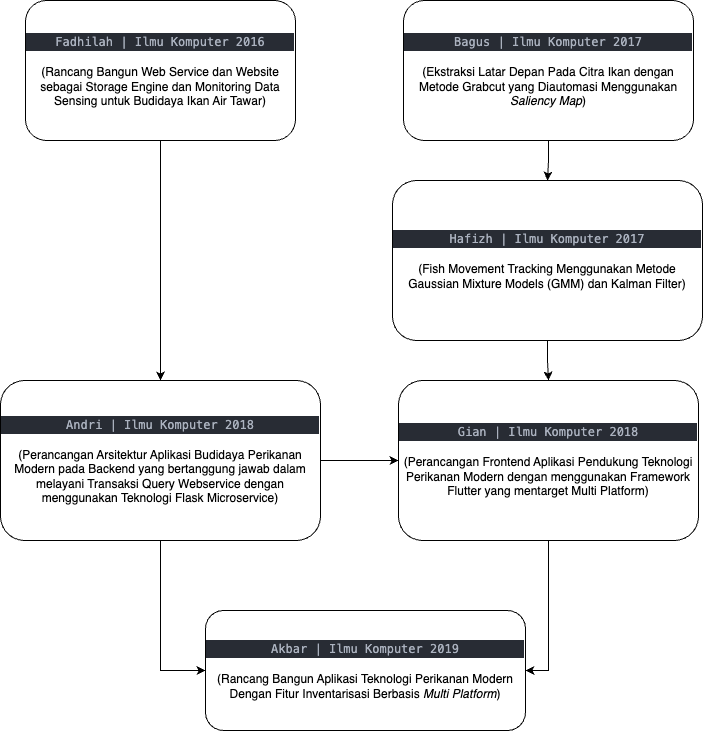
\includegraphics[width=0.7\textwidth]{gambar/research_tree.png}
	\caption{Diagram Alur Penelitian \textit{Aquaculture}}
\end{figure}

Pada diagram diatas, dapat dilihat urutan arah dari topik penelitian Aquaculture. Penelitian pertama kali dimulai oleh \citep{fadhil2021} dengan mengembangkan sebuah web service serta website yang berfungsi sebagai Storage Engine dan Monitoring Data Sensing untuk digunakan pada Budidaya Perikanan Air Tawar sebagai media penyimpanan data-data sensing dari sensor yang dikirimkan ke sistem serta memonitoringnya dalam bentuk table dan grafik real-time serta penelitian yang dilakukan oleh \citep{bagus2022} dengan tujuan untuk membangun sistem deteksi objek pada citra ikan dengan metode GrabCut yang telah diautomasi menggunakan \textit{saliency map}. 

Penelitian \citep{bagus2022} kemudian dilanjutkan oleh \citep{hafiz2021} yaitu merancang dan membangun sebuah sistem yang dapat melakukan pelacakan pergerakan ikan dengan menggunakan metode GMM dan Kalman Filter. Sementara penelitian \citep{fadhil2021} belum diterapkan pada aplikasi riset Aquaculture dalam waktu dekat sehingga penelitian yang dibuat oleh \citep{andri2022} dilakukan dengan membuat web service juga yang bertujuan untuk melayani transaksi query berupa monitoring budidaya perikanan yang dibarengi dengan penelitian \citep{gian2022} pada bagian perancangan \textit{frontend} sebagai pendukung pada aplikasi yang dikembangkan.

Dalam penelitian yang sudah berjalan ini, penulis mengembangkan penelitian yang dilakukan oleh \citep{andri2022} dan \citep{gian2022} dengan membuat fitur baru yaitu manajemen inventaris serta penentuan harga jual ikan dan penentuan upah pembudidaya ikan.

\section{Metode Penentuan Nilai Jual}

% Dalam beberapa skenario, harga jual ditentukan oleh pedagang kepada pembudidaya. Harga ini dijamin lebih kecil dibanding harga retail, karena pedagang akan mengambil keuntungan dari itu. Jika dimisalkan T adalah harga jual minimum agar pembudidaya tidak rugi, $W_{feed}$ sebagai total pakan yang diberikan dan P adalah harga satuan pakan. Maka hubungan dari variabel-variabel tersebut adalah sebagai berikut.
% \begin{equation}
%     \begin{split}
% 		T
% 		&= W_{feed} \times P
%     \end{split}
% \end{equation}

% Rumus ini didasari oleh konversi antara kilogram pakan menjadi pertambahan berat sebagian besar bervariasi tergantung pada kasus tertentu. Terlepas dari itu ditentukan oleh semakin tinggi asupan protein, maka semakin rendah tingkat konversinya. Jika konversi ini dikaitkan sebagai Food Conversion Ratio  (FCR) yang dimana $W_{fish}$ sebagai total berat dari semua ikan yang dipanen.
% \begin{equation}
%     \begin{split}
% 		FCR
% 		&= W_{feed } \div W_{fish}
%     \end{split}
% \end{equation}

% Oleh karena itu, pembudidaya harus mencatat berapa banyak kilogram pakan yang diberikan sampai musim panen dari tiap kolam untuk menemukan nilai FCR-nya. Dalam masalah yang lebih kompleks, jika pakan memungkinkan datang dari berbagai sumber yang berhubungan dengan variasi asupan protein, FCR tidak dapat digunakan untuk menentukan hubungan antara jumlah pakan dan pertambahan berat.  Maka dari itu, sangat direkomendasikan untuk pembudidaya agar menggunakan satu sumber asupan protein tiap musim panen. Karena FCR sudah diketahui, selama musim panen berikutnya pembudidaya bisa memperkirakan berapa banyak pakan yang dibutuhkan untuk membuat ikan agar tumbuh sampai ukuran yang ditargetkan.
% \begin{equation}
%     \begin{split}
% 		W_{fish}
% 		&= W_{feed} \div FCR
%     \end{split}
% \end{equation}

% Dengan itu bisa digunakan dalam mencari total jumlah pakan yang dibutuhkan untuk membuat ikan agar tumbuh sampai ukuran yang ditargetkan. 
% \begin{equation}
%     \begin{split}
% 		W_{feed}
% 		&= W_{fish} \times FCR
%     \end{split}
% \end{equation}

% Jika persamaan 4 dikembangkan dengan memasukkan dua variabel yaitu $W_i$ sebagai berat ikan dan n sebagai jumlah ikan, maka persamaan akan menjadi seperti berikut.
% \begin{equation}
%     \begin{split}
% 		W_{fish}
% 		&= \sum_{i=1}^n \times W_i
%     \end{split}
% \end{equation}

% Namun, menggunakan persamaan 5 akan mematikan tujuan dari persamaan 4, karena jika ingin menghitung pemakaian pakan diharuskan untuk menilai masing-masing ikan secara individu yang dimana itu tidak praktis. Jika menggunakan variabel $W_{af}$ sebagai rata-rata dari berat ikan, maka persamaan akan menjadi sebagai berikut.
% \begin{equation}
%     \begin{split}
% 		W_{af}
% 		&= \frac{\sum_{i=1}^n \times W_i}{n}
%     \end{split}
% \end{equation}

% Sekarang dapat dengan mudah mencari perkiraan konsumsi pakan untuk musim panen berikutnya dengan persamaan,
% \begin{equation}
%     \begin{split}
% 		W_{feed}
% 		&= W_{af} \times n \times FCR
%     \end{split}
% \end{equation}


% Jika persamaan 1 diupdate sehingga dapat ditemukan harga sesuai dengan persamaan,
% \begin{equation}
%     \begin{split}
% 		T_{unit}
% 		&= \frac{T}{n}
%     \end{split}
% \end{equation}

% Persamaan itu juga merujuk pada jumlah perdagangan dalam kilogram, oleh karena itu
% \begin{equation}
%     \begin{split}
% 		k
% 		&= \frac{1kg}{W_{af}}
%     \end{split}
% \end{equation}

% \begin{equation}
%     \begin{split}
% 		T_k
% 		&= T_{unit} \times k
%     \end{split}
% \end{equation}

% Sebagai contoh, dimisalkan mata uang yang digunakan adalah koin lalu FCR bernilai 1.5, ukuran target panen adalah 4 ikan per kilogram, di kolam terdapat 1000 ikan, dan harga pakan mencapai 10 koin.

% Dari data tersebut, dapat diketahui $W_{af}$ = 1/4 kg, n = 1000. Karena itu, $W_{feed}$ bernilai 375 kg yang harus dipersiapkan. Selanjutnya, pembudidaya tidak bisa menjual semua hasil panen ikan seharga dibawah T = 3750 koin atau dibawah 15 koin per kilogram.

% Persamaan 1 sampai 10 memungkinan jika FCR konstan dengan treatment yang sama dan asupan protein yang sama. Seperti yang sudah dilakukan diawal, pembudidaya harus mengandalkan satu sumber protein tetapi untuk mempertahankan hal ini sulit dilakukan. Karena itu, PER (Protein Efficiency Ratio) diketahui untuk menentukan rasio massa tubuh yang diperoleh dengan gram protein yang dikonsumsi. Disini variabel $P_{feed}$ mendefinisikan asupan gram protein.
% \begin{equation}
%     \begin{split}
% 		PER
% 		&= \frac{W_{fish}}{P_{feed}}
%     \end{split}
% \end{equation}

% Pada formula tersebut, menggantikan $W_{feed}$ pada persamaan 2 dengan $P_{feed}$ akan memberikan bentuk variabel yang sama namun struktur variabel yang terbalik. Hal ini juga memberikan kemungkinan untuk mencampur beberapa sumber protein yang berbeda dengan formula berikut.
% \begin{equation}
%     \begin{split}
% 		PER
% 		&= \frac{W_{fish}}{P^1_{feed} + P^2_{feed} + \dots + P^k_{feed}}
%     \end{split}
% \end{equation}

% \begin{equation}
%     \begin{split}
% 		PER
% 		&= \frac{W_{fish}}{\sum_{i=1}^k \times P^i_{feed}}
%     \end{split}
% \end{equation}

% Variabel k mengartikan jumlah dari sumber protein yang berbeda. Hal ini juga dapat dilakukan pada FCR dan T sebagai berikut.
% \begin{equation}
%     \begin{split}
% 		FCR
% 		&= \frac{\sum_{i=1}^k \times W^k_{feed}}{W_{fish}}
%     \end{split}
% \end{equation}
% \begin{equation}
%     \begin{split}
% 		T
% 		&= \sum_{i=1}^k \times W^k_{feed} \times P
%     \end{split}
% \end{equation}

% Pada persamaan 15, hanya memodelkan harga jual minimum barang perikanan agar terhindar dari kerugian. Karena itu, untuk mendapatkan keuntungan diperlukan model yang baru. Disini variabel $T_p$ melambangkan dagangan yang memberikan keuntungan dan $F_g$ sebagai pendapatan pembudidaya.
% \begin{equation}
%     \begin{split}
% 		T_p
% 		&= T + F_g
%     \end{split}
% \end{equation}

% $F_g$ merepresentasikan berapa banyak jam kerja yang dilakukan pembudidaya untuk membudidayakan ikan. Hal ini dapat dijelaskan lebih rinci dalam
% \begin{equation}
%     \begin{split}
% 		F_g
% 		&= D \times S
%     \end{split}
% \end{equation}

% Dimana D mengartikan berapa banyak hari pembudidaya bekerja sampai musim panen dan S mengartikan upah yang mewakili pendapatan pekerjaan. Dalam berbudidaya, merupakan hal umum bagi pembudidaya ikan untuk menghabiskan waktu seharian penuh untuk mengembangkan dan memantau kolam, karena itu representasi hari lebih ideal. Sebab itu, pembudidaya yang lebih banyak menghabiskan waktunya sampai musim panen tiba harus mendapatkan pendapatan yang sesuai.

% Persamaan 15 berlaku jika budidaya ikan membudidayakan ikan tradisional secara tradisional. Dalam sistem intensif aquaculture khususnya BFT, dibutuhkan variabel yang mewakili biaya tambahan yang dikeluarkan untuk penggunaan teknologi. Variabel ${C_i}$ merepresentasikan masing-masing biaya tambahan yang dikeluarkan dalam BFT untuk keseluruhan musim kawin.
% \begin{equation}
%     \begin{split}
% 		T
% 		&= \sum_{i=1}^k \times W^k_{feed} \times P + \sum_{i=1}^l \times C_i
%     \end{split}
% \end{equation}

% Variabel $C_i$ dapat dijabarkan sebagai berikut.

% \begin{itemize}
% 	\item $C_1$ = Bahan baku (termasuk pakan dan bahan budidaya)
% 	\item $C_2$ = Listrik (dihitung dalam per kolam)
% 	\item $C_3$ = Tenaga kerja (dihitung 3-5 jam / orang serta dibagi dengan jumlah kolam)
% 	\item $C_4$ = Benih ikan
% \end{itemize}

Dalam menyimpan bahan baku pada inventaris, bahan baku tersebut akan mengalami penurunan karena bahan baku mempunyai masa kadaluarsa. Maka dari itu, dapat dimisalkan jika per bulan bahan baku tersebut mengalami penurunan kualitas sebesar 25\% dari harga belinya, maka dalam 4 bulan bahan baku tersebut akan kadaluarsa dan sudah tidak lagi berharga. Namun, skala penurunan tersebut bervariasi tergantung pada jenis bahan baku yang digunakan. Variabel $W_p$ mewakili harga dari bahan baku yang digunakan dan variabel $\alpha$ mewakili skala depresiasi per bulan dari bahan baku yang digunakan. Formula depresiasi dapat dibuat menjadi persamaan berikut.

\begin{equation}
    \begin{split}
		W_p
		&= W_p - \alpha \times W_p
    \end{split}
\end{equation}

Ketika hasil ikan sudah bisa dipanen, maka harga ikan sementara yang bisa digunakan dapat dihitung dengan rumus berikut.

\begin{equation}
    \begin{split}
		T
		&= \frac{\sum_{i=1}^3 C_i + \frac{C_l}{n}}{N}
    \end{split}
\end{equation}

\begin{itemize}
	\item T = Harga jual ikan
	\item $C_1$ = Harga total benih selama musim berjalan
	\item $C_2$ = Harga total pakan selama musim berjalan
	\item $C_3$ = Harga total bahan budidaya selama musim berjalan
	\item $C_l$ = Harga tagihan listrik
	\item n = Jumlah kolam
	\item N = Jumlah ikan yang hidup
\end{itemize}

Harga dari perhitungan tersebut dapat digunakan oleh pembudidaya untuk menjadi harga dasar dalam penjualannya. Tentunya harga tersebut hanya merupakan harga panen dan pembudidaya tidak wajib menggunakan harga tersebut dalam transaksi.

\section{Tahapan Penelitian}

\begin{figure}[H]
	\centering
	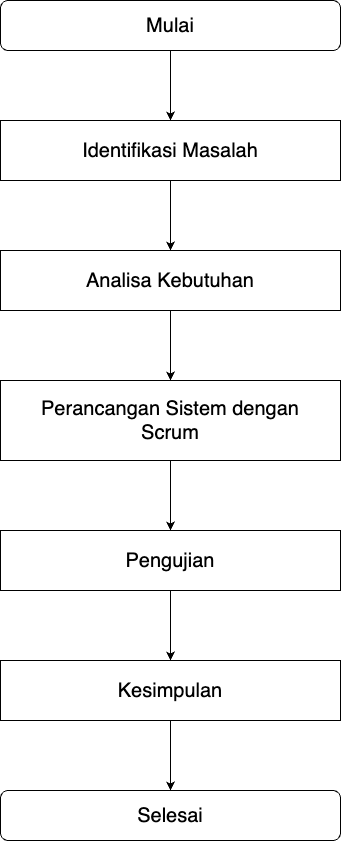
\includegraphics[width=0.35\textwidth]{gambar/tahapan_penelitian.png}
	\caption{Alur Tahapan Penelitian}
\end{figure}

Desain penelitian adalah alur yang dijalankan selama masa pengembangan aplikasi. Pada \textbf{Gambar 3.2}, terdapat desain penelitian yang digunakan dalam pembuatan aplikasi ini dengan metode Scrum.

% \section{Analisa Arsitektur Fitur}

% Pada penelitian aplikasi yang sudah dikembangkan sebelumnya, terdapat use case yang menjelaskan konsep dari aplikasi yang ada pada gambar dibawah ini.

% \begin{figure}[H]
% 	\centering
% 	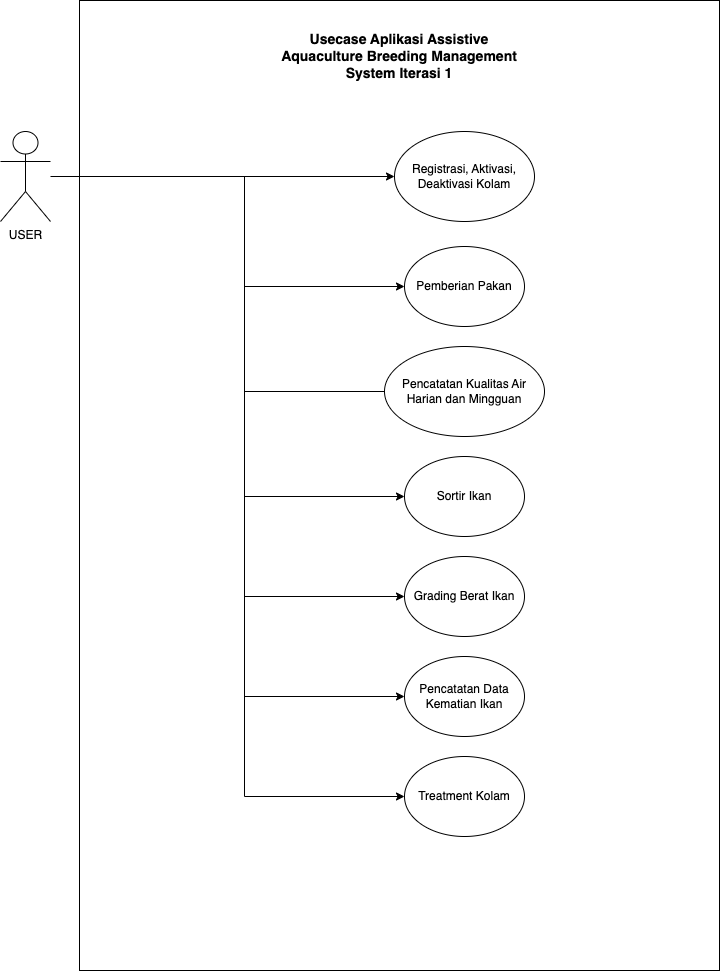
\includegraphics[width=0.8\textwidth]{gambar/usecase_iterasi_1.png}
% 	\caption{Use Case Fitur Aplikasi pada Iterasi 1}
% \end{figure}

% Dari diagram use case tersebut, terdapat dua jenis pengguna yaitu user dan admin. User dan admin memiliki fitur yang sama dalam aplikasi tersebut, yang membedakan antara user dan admin adalah skala prioritas dari aplikasi. Sisi admin memungkinkan pengguna dapat mengatur lebih banyak fitur yang ada pada aplikasi dan mendapatkan akses untuk mengatur user non-admin. Fitur yang disediakan aplikasi dijelaskan sebagai berikut.

% \begin{enumerate}
% 	\item \textbf{Registrasi, Aktivasi, Deaktivasi Kolam} = Fitur ini digunakan untuk mendaftarkan kolam yang akan dijadikan tempat budidaya ikan, kemudian fitur aktivasi dan deaktivasi kolam digunakan untuk mengontrol kolam yang sedang berjalan.
% 	\item \textbf{Pemberian Pakan} = Fitur ini digunakan untuk mencatat data pakan yang diberikan pada kolam ikan di budidaya yang sedang berlangsung.
% 	\item \textbf{Pencatatan Kualitas Air Harian dan Mingguan} = Fitur ini digunakan untuk mencatat kualitas air dari kolam di budidaya yang sedang berjalan dengan rentang waktu harian dan mingguan.
% 	\item \textbf{Sortir Ikan} = Fitur ini digunakan untuk mengatur perpindahan ikan ke kolam lain.
% 	\item \textbf{Grading Berat Ikan} = Fitur ini digunakan untuk mengatur ekosistem ikan berdasarkan berat agar mendapatkan keseragaman ukuran ikan dan meningkatkan efektivitas pemberikan pakan kepada ikan.
% 	\item \textbf{Pencatatan Data Kematian Ikan} = Fitur ini digunakan untuk mencatat angka kematian ikan jika terdapat ikan yang mati ketika budidaya sedang berjalan.
% 	\item \textbf{Treatment Kolam} = Fitur ini digunakan untuk melakukan pengaturan terhadap kolam ikan pada budidaya yang sedang berjalan.
% \end{enumerate}

\section{Analisa Kebutuhan}

Pada pengembangan aplikasi lanjutan ini, fitur yang ditambahkan adalah fitur manajemen inventaris serta fitur pembukuan. Fitur pencatatan inventaris merupakan fitur yang akan ada pada aplikasi yang berguna untuk para pembudidaya ikan mencatat semua hal yang berhubungan dengan budidaya perikanannya. Hal-hal yang dapat dicatat oleh pembudidaya pada fitur ini seperti bahan baku (termasuk pakan dan bahan budidaya), penggunaan listrik, benih, serta aset yang digunakan selama masa budidaya dilakukan.

Selain mencatat inventaris pada musim budidaya, fitur pencatatan inventaris ini juga dapat menentukan rekomendasi harga jual dari ikan yang dipanen oleh pembudidaya ikan berdasarkan perhitungan dari pengeluaran biaya selama musim budidaya berjalan. Beberapa fitur yang sudah ada di penelitian sebelumnya juga harus diperbarui dengan adanya manajemen inventaris ini seperti panen, pemberian pakan, sortir ikan, serta treatment kolam.

Kemudian untuk fitur pembukuan berguna untuk pembudidaya ikan melihat riwayat musim budidaya yang sudah mereka jalankan. Terdapat beberapa rincian yang ditampilkan seperti biaya pengeluaran sampai berapa total ikan yang terpanen pada musim budidaya tersebut.

Fitur-fitur tersebut dapat dibuat menjadi use case pada \textbf{Gambar 3.3}. Pada use case tersebut, font warna hitam merupakan fitur yang sudah ada pada penelitian sebelumnya yang tidak berubah dan font warna cokelat merupakan fitur sebelumnya yang akan diperbarui pada penelitian ini. Sementara itu, untuk font warna hijau merupakan fitur baru yang akan tersedia pada aplikasi dan dikembangkan pada penelitian ini.

\begin{figure}[H]
	\centering
	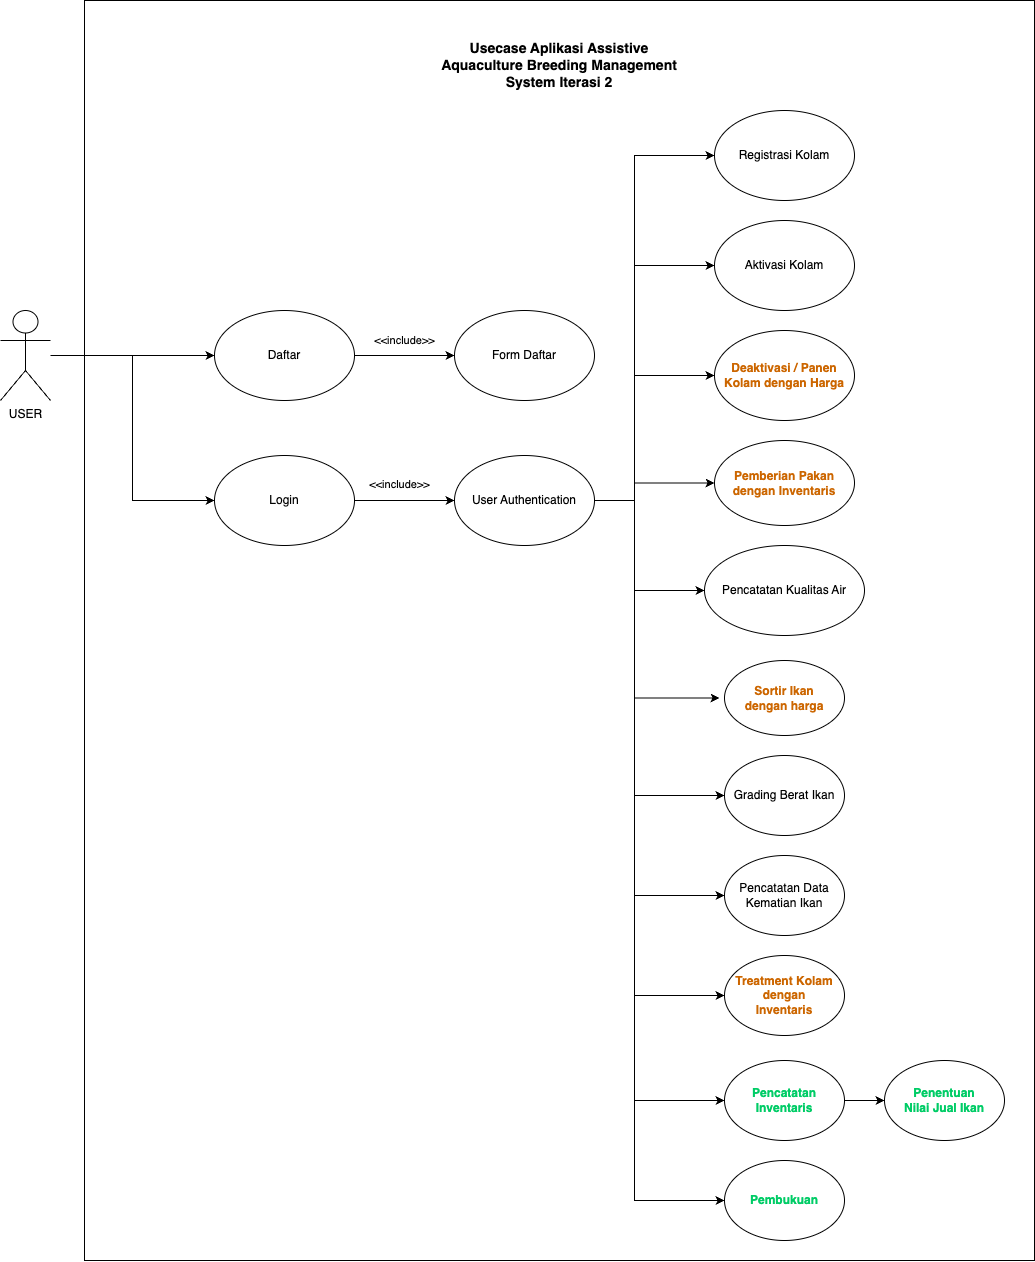
\includegraphics[width=1\textwidth]{gambar/usecase_iterasi_2.png}
	\caption{Use Case Aplikasi}
\end{figure}

\section{Perancangan Sistem}

Pada aplikasi yang akan dibuat pada penelitian ini dikembangkan dengan metode Scrum. Beberapa komponen scrum seperti product backlog, sprint backlog, daily sprint, serta daily meet digunakan agar terwujudnya ketertiban dalam masa pengembangan aplikasi. Berikut penjelasan dari masing-masing elemen yang ada pada metode Scrum.

\begin{figure}[H]
	\centering
	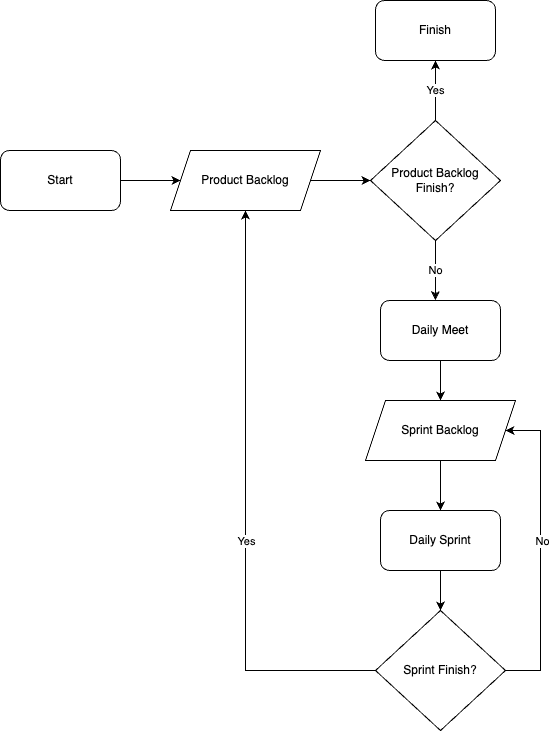
\includegraphics[width=0.8\textwidth]{gambar/scrum.png}
	\caption{Tahapan Perancangan Sistem dengan Metode Scrum}
\end{figure}

\begin{enumerate}
	\item Product Backlog
	
	Product Backlog adalah tugas-tugas yang \textbf{akan} dijalankan pada penelitian dan hal yang pertama kali dilakukan sebelum memulai riset. Daftar tugas yang ada pada Product Backlog ini akan dipindahkan pada Sprint Backlog tergantung pada skala prioritas dari task itu sendiiri. Berikut adalah tabel dari Product Backlog yang sudah berjalan.

	\begin{table}[H]	
		\begin{center}
			\caption{Product Backlog}
			\label{tab:table5}
			\begin{tabular}{|c|m{17em}|c|c|}
			\hline
			\textbf{No} & \textbf{Stories} & \textbf{Sprint} & \textbf{Status} \\
			\hline
			1 & Pencatatan inventaris & 1, 2 & On Progress \\
			\hline
			2 & Aktivasi kolam dengan inventaris & - & Uncomplete \\
			\hline
			3 & Depresiasi aset dalam inventaris & - & Uncomplete \\
			\hline
			4 & Pemberian pakan yang terkoneksi dengan inventaris & - & Uncomplete \\
			\hline
			5 & Treatment kolam yang terkoneksi dengan inventaris & - & Uncomplete \\
			\hline
			6 & Sortir termasuk harga nilai jual ikan & - & Uncomplete \\
			\hline
			7 & Panen termasuk harga nilai jual ikan & - & Uncomplete \\
			\hline
			8 & Pembukuan pencatatan pengeluaran per musim budidaya & - & Uncomplete \\
			\hline
			\end{tabular}
		\end{center}
	\end{table}	

	\item Sprint Backlog
	
	Sprint Backlog adalah daftar tugas yang \textbf{harus} dijalankan selama masa Sprint berlangsung. Tugas yang ada pada Sprint Backlog bersifat fleksibel seiring dengan berjalannya Sprint.

	\item Sprint
	
	Progres sprint dilaksanakan ketika list task pada sprint backlog sudah disepakati bersama. Periode pengerjaan sprint bervariasi tergantung pada kesulitan task dari sprint backlog tersebut.

	\begin{enumerate}
		\item \textbf{Sprint 1}
		
		Sprint 1 dilaksanakan pada tanggal 07 Maret 2023 - 29 Maret 2023. Detail dari Sprint 1 ini adalah mengerjakan tugas yang ada pada Sprint 1 Backlog di tabel berikut.

		\begin{table}[H]	
			\begin{center}
				\caption{Sprint 1 Backlog}
				\label{tab:table6}
				\begin{tabular}{|c|c|m{13em}|c|}
				\hline
				\textbf{No} & \textbf{Stories} & \textbf{Task} & \textbf{Status} \\
				\hline
				1 & \multirow{2}{10em}{Fitur pencatatan inventaris} & - Membuat skema database dari pencatatan inventaris & Complete \\
				&  & - Membuat integrasi skema database dengan skema database sebelumnya & Complete \\
				&  & - Membuat mockup dari fitur inventaris & Complete \\
				\hline
				\end{tabular}
			\end{center}
		\end{table}

		Berikut merupakan skema database yang mewakili fitur inventaris dapat dilihat pada \textbf{Gambar 3.5} berikut.
		
		\begin{figure}[H]
			\centering
			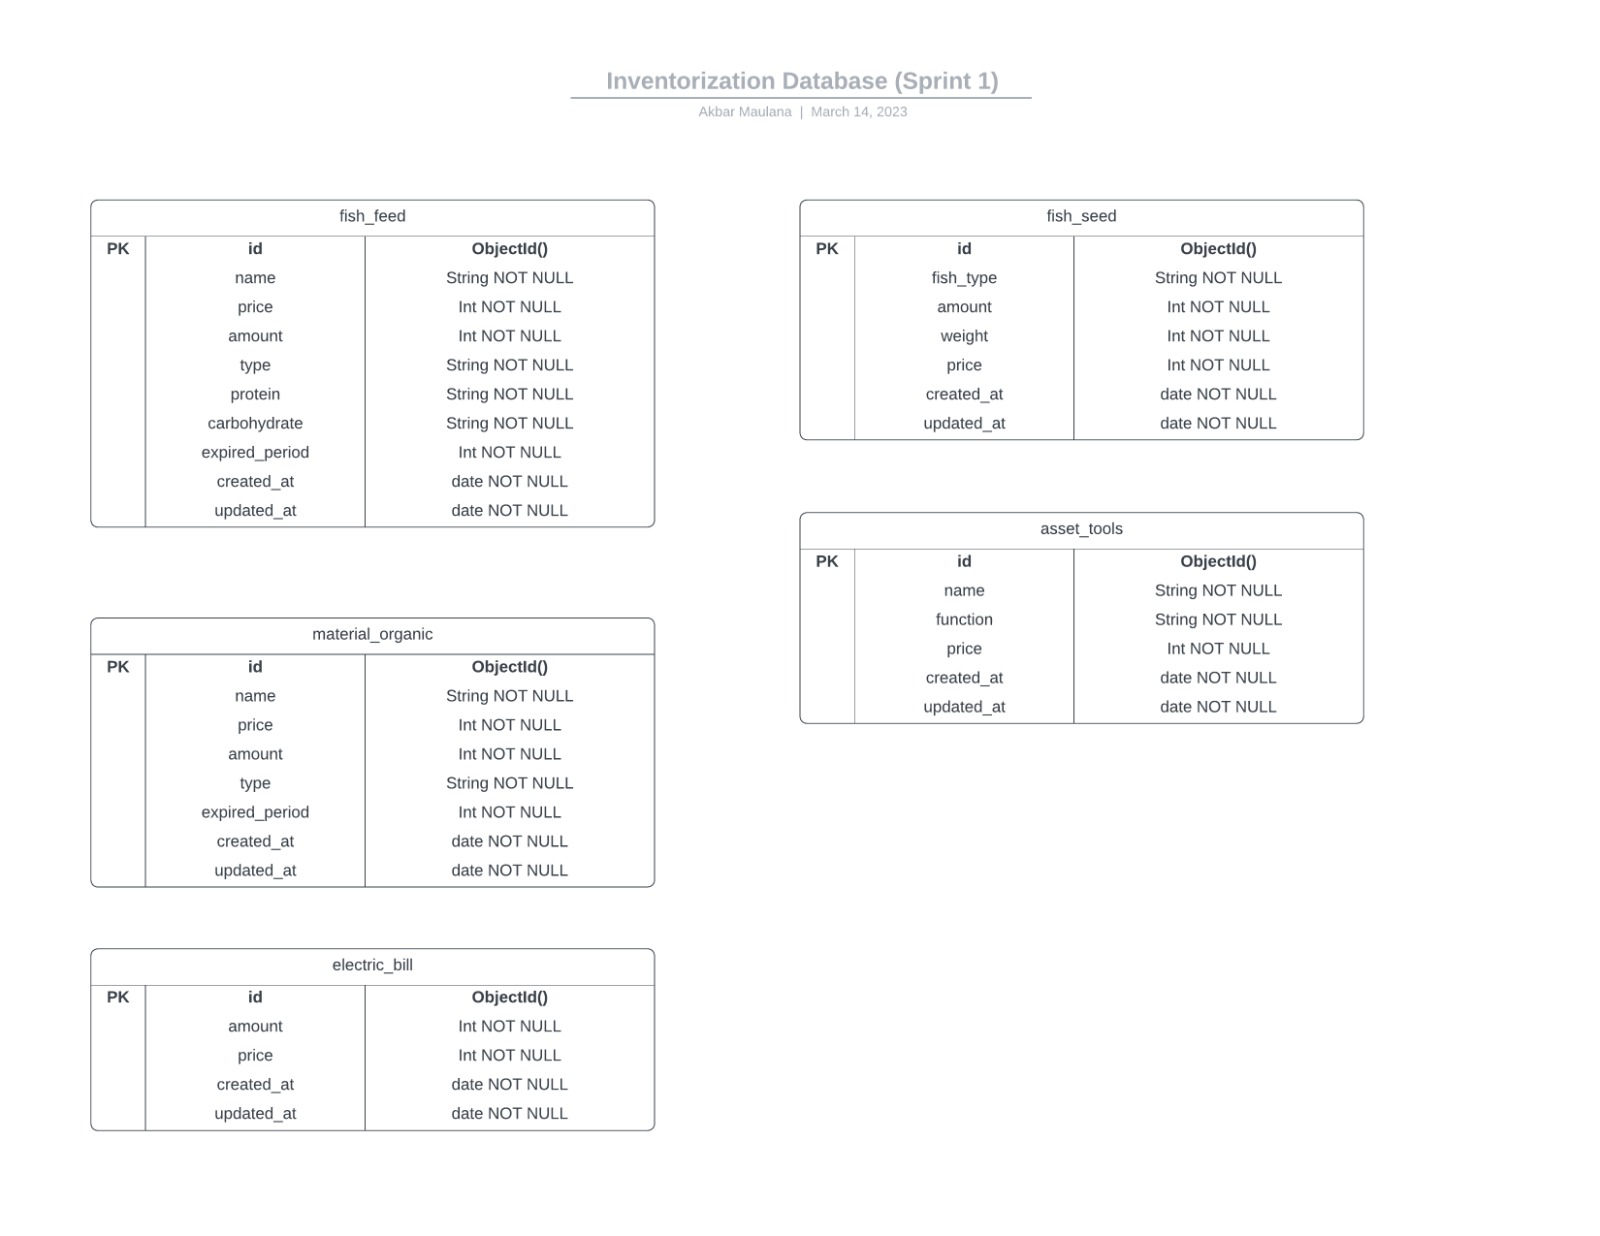
\includegraphics[width=1\textwidth]{gambar/sprint1/sprint1_inventaris_database.jpeg}
			\caption{Skema Database Fitur Inventaris}
		\end{figure}
	
		Dari skema database tersebut, terdapat lima opsi kategori inventaris yang sudah dijelaskan sebelumnya. Pada skema database ini, masing-masing kategori memiliki kebutuhan yang berbeda antara lain.
	
		\begin{enumerate}
			\item fish\_feed (Pakan Ikan)
			\item material\_organic (Bahan Organik)
			\item electric\_bill (Tagihan Listrik)
			\item fish\_seed (Benih Ikan)
			\item asset\_tools (Peralatan)
		\end{enumerate}
	
		Dalam tabel database tersebut, pada kolom pertama terdapat jenis \textit{key} yang dijadikan patokan dalam tabel database tersebut. Kemudian kolom kedua dan ketiga merupakan hubungan antara nama data dan tipe data yang mewakili nama data tersebut.
	
		Setelah skema database dari inventaris telah dibuat, tabel-tabel database tersebut harus diintegrasikan dengan skema database sebelumnya untuk menyesuaikan kebutuhan fitur yang akan dibuat nantinya. Berikut merupakan skema database yang telah diintegrasikan dengan skema database dari inventaris dapat dilihat pada \textbf{Gambar 3.5}.
	
		\begin{figure}[H]
			\centering
			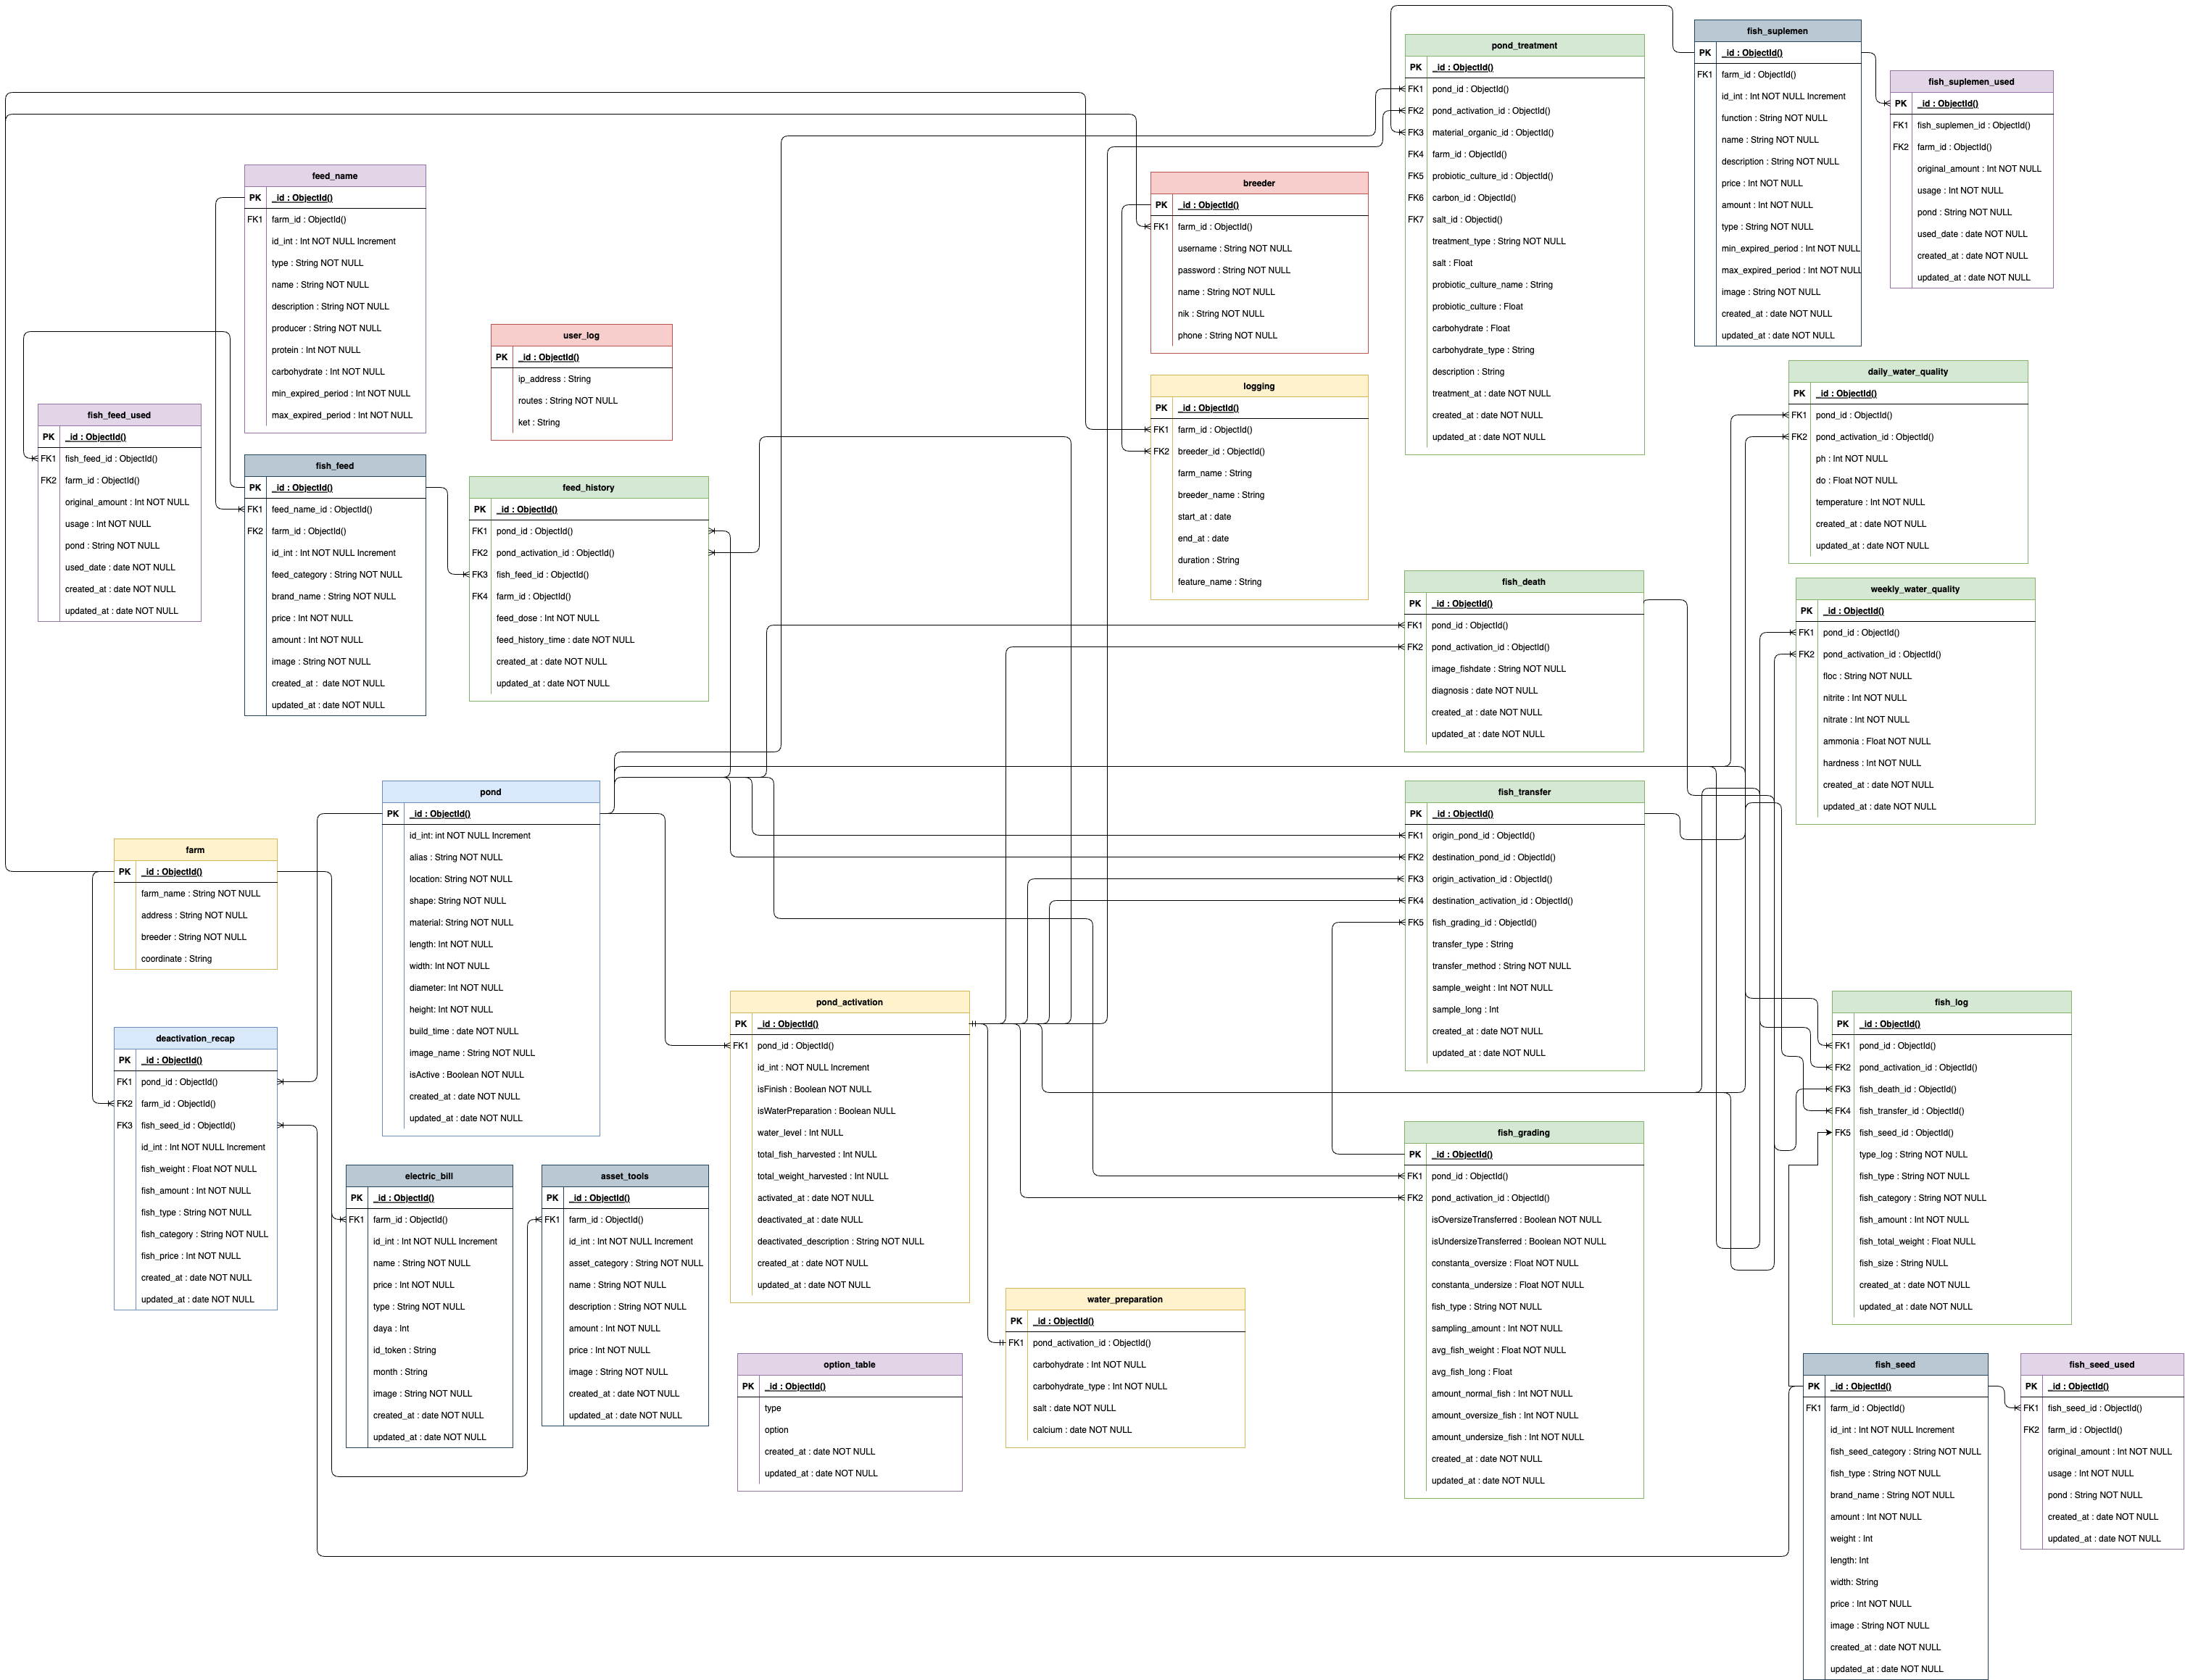
\includegraphics[width=1\textwidth]{gambar/sprint1/sprint1_skema_database.png}
			\caption{Integrasi Skema Database Inventaris dengan Skema Database Iterasi 1}
		\end{figure}

		Dari integrasi diatas, tabel fish\_feed diintegrasikan dengan tabel feed\_type yang digunakan untuk input pakan dan tabel material\_organic diintegrasikan dengan tabel pond\_treatment karena dalam fitur treatment kolam diperlukan data dari tabel material organik tersebut. Lalu tabel fish\_seed diintegrasikan dengan tabel pond\_activation dan fish\_log untuk aktivasi kolam dan perhitungan jumlah ikan. Sementara itu, tabel electric\_bill dan asset\_tools merupakan individu yang tidak terintegrasi dengan tabel yang lain. Hal ini dikarenakan tabel tersebut hanya untuk menyimpan datanya saja dan tidak digunakan di dalam fitur.

		Berikut merupakan mockup dari fitur inventaris yang mencakup skema database sebelumnya.

		\begin{figure}[H]
			\minipage{0.32\textwidth}
			  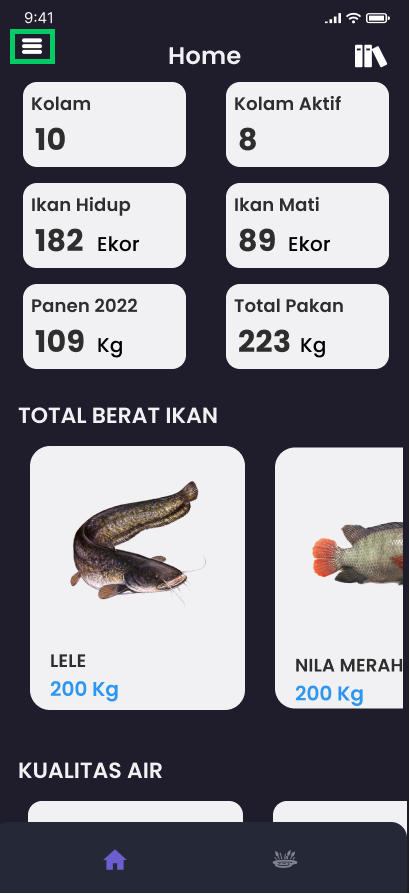
\includegraphics[width=\linewidth]{gambar/sprint1/mockup_dashboard.png}
			  \caption{Halaman Dashboard}
			\endminipage\hfill
			\minipage{0.32\textwidth}%
			  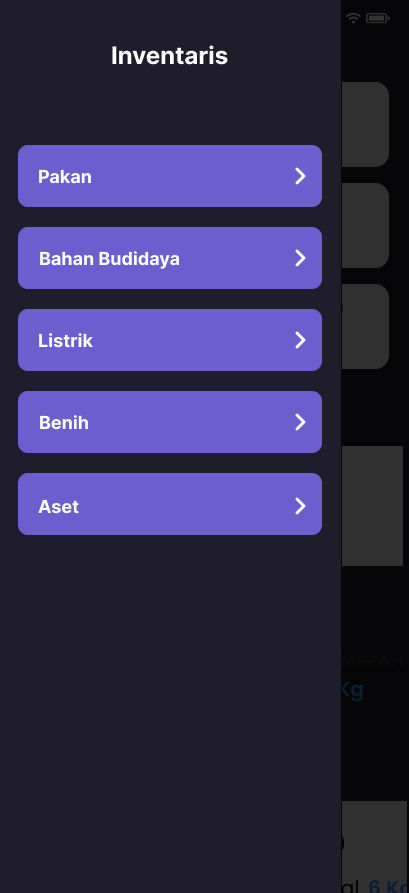
\includegraphics[width=\linewidth]{gambar/sprint1/mockup_home.png}
			  \caption{Halaman Menu Inventaris}
			\endminipage
		\end{figure}

		Pada halaman dashboard, dipojok kiri atas terdapat ikon \textit{hamburger} atau list yang ketika ditekan akan menampilkan halaman menu inventaris seperti \textbf{Gambar 3.8}. Masing-masing list menu yang ada pada halaman menu inventaris memiliki fungsi-fungsi yang sesuai dengan skema inventaris.

		\begin{figure}[H]
			\minipage{0.32\textwidth}
			  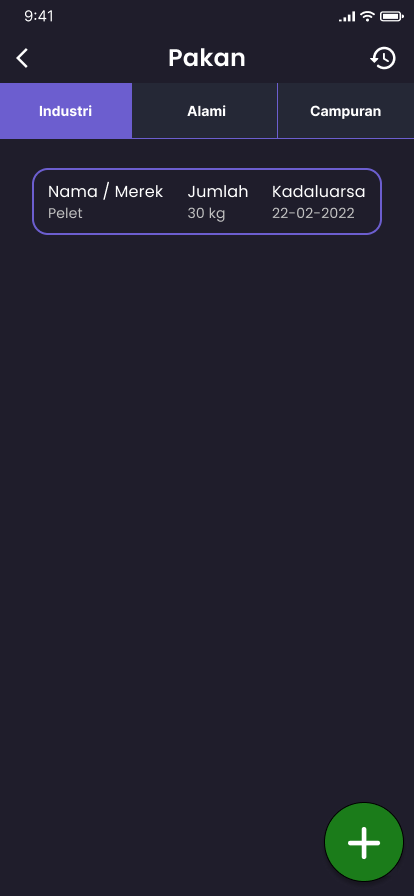
\includegraphics[width=\linewidth]{gambar/sprint1/mockup_detail_feed.png}
			  \caption{Halaman Data Inventaris Pakan}
			\endminipage\hfill
			\minipage{0.32\textwidth}
			  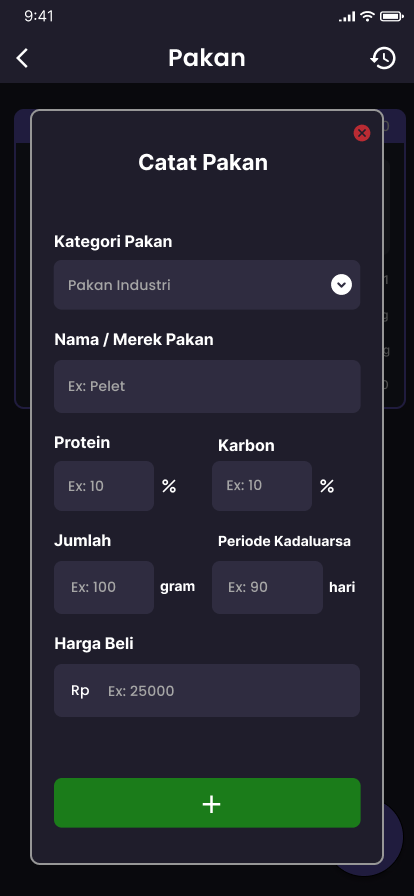
\includegraphics[width=\linewidth]{gambar/sprint1/mockup_input_feed.png}
			  \caption{Halaman Input Inventaris Pakan}
			\endminipage\hfill
			\minipage{0.32\textwidth}%
			  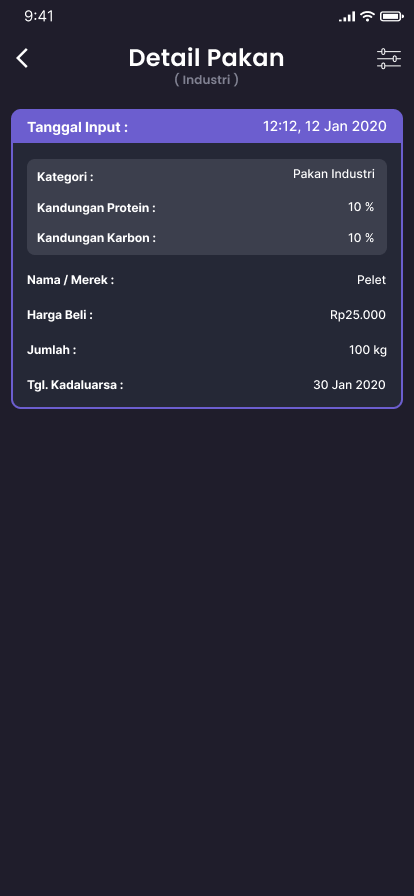
\includegraphics[width=\linewidth]{gambar/sprint1/mockup_list_feed.png}
			  \caption{Halaman Detail Inventaris Pakan}
			\endminipage
		\end{figure}

		Jika pada halaman menu inventaris sebelumnya dipilih menu "Pakan", maka akan masuk ke halaman data inventaris pakan. Pada halaman ini terdapat 3 jenis pakan yaitu pakan industri (pelet), alami (tumbuh-tumbuhan), serta campuran (tepung, terigu, dll). Masing-masing jenis pakan memiliki detail data yaitu nama atau merek pakan, total jumlah pakan yang tersedia, serta tanggal kadaluarsa dari pakan tersebut.

		Tombol (+) yang ada di pojok kanan bawah akan mengarahkan ke halaman input dari inventaris pakan. Disini diberikan form input yang beragam seperti yang ada pada \textbf{Gambar 3.10}.

		Sementara tombol riwayat yang ada di pojok kanan atas akan mengarahkan ke halaman detail dari inventaris pakan. Di halaman ini ditampilkan detail pemasukkan pakan ke sistem inventaris.

		\begin{figure}[H]
			\minipage{0.32\textwidth}
			  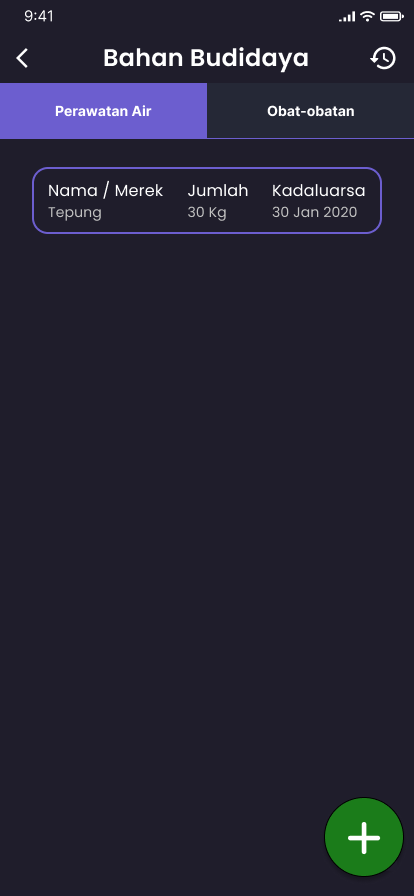
\includegraphics[width=\linewidth]{gambar/sprint1/mockup_detail_materials.png}
			  \caption{Halaman Data Inventaris Bahan Budidaya}
			\endminipage\hfill
			\minipage{0.32\textwidth}
			  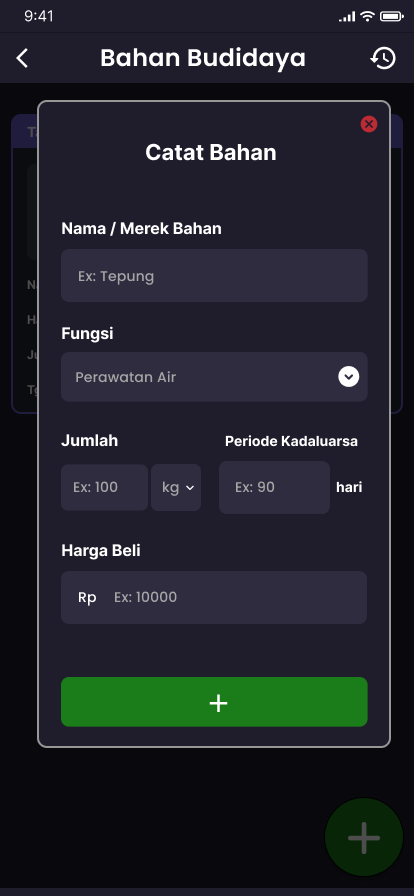
\includegraphics[width=\linewidth]{gambar/sprint1/mockup_input_materials.png}
			  \caption{Halaman Input Inventaris Bahan Budidaya}
			\endminipage\hfill
			\minipage{0.32\textwidth}%
			  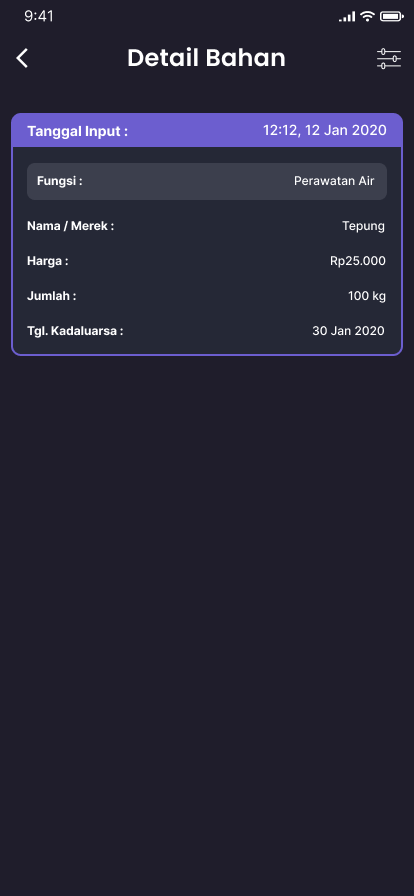
\includegraphics[width=\linewidth]{gambar/sprint1/mockup_list_materials.png}
			  \caption{Halaman Detail Inventaris Bahan Budidaya}
			\endminipage
		\end{figure}

		Jika pada halaman menu inventaris sebelumnya dipilih menu "Bahan Budidaya", maka akan masuk ke halaman data inventaris bahan budidaya. Pada halaman ini terdapat 2 jenis bahan budidaya yang dibagi berdasarkan fungsi yaitu perawatan air dan obat-obatan (Methylene Blue, dll). Sama seperti pada inventaris pakan, masing-masing jenis bahan budidaya memiliki detail data yaitu nama atau merek, total jumlah yang tersedia, serta tanggal kadaluarsa.

		Sama seperti halaman inventaris pakan, tombol (+) mengarahkan ke halaman input seperti \textbf{Gambar 3.13} dan tombol riwayat akan mengarahkan ke halaman detail inventaris seperti pada \textbf{Gambar 3.14}.

		\begin{figure}[H]
			\minipage{0.32\textwidth}
			  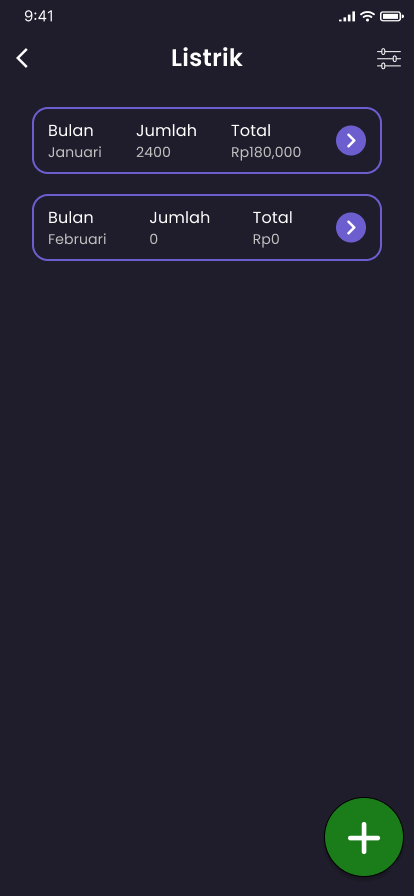
\includegraphics[width=\linewidth]{gambar/sprint1/mockup_detail_electric.png}
			  \caption{Halaman Data Inventaris Tagihan Listrik}
			\endminipage\hfill
			\minipage{0.32\textwidth}
			  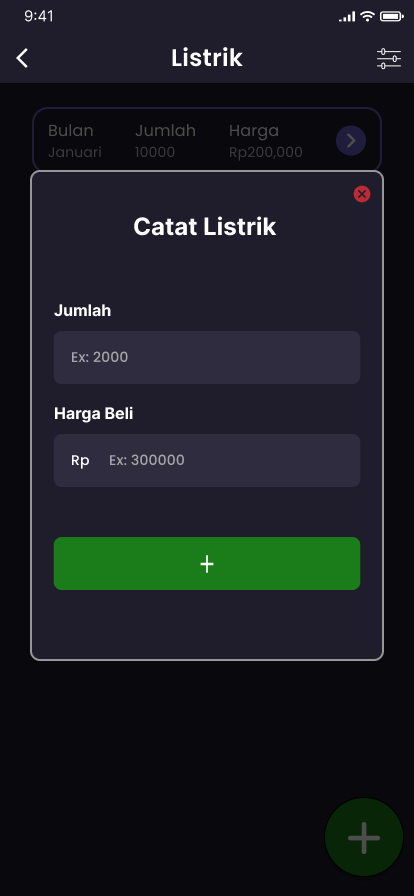
\includegraphics[width=\linewidth]{gambar/sprint1/mockup_input_electric.png}
			  \caption{Halaman Input Inventaris Tagihan Listrik}
			\endminipage\hfill
			\minipage{0.32\textwidth}%
			  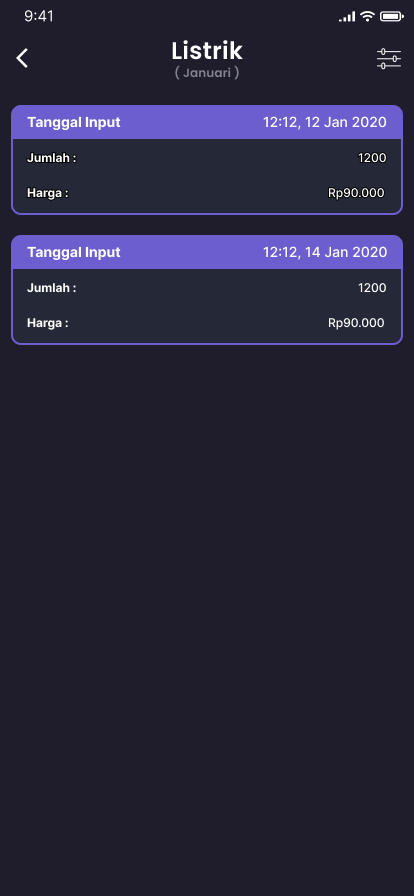
\includegraphics[width=\linewidth]{gambar/sprint1/mockup_list_electric.png}
			  \caption{Halaman Detail Inventaris Tagihan Listrik}
			\endminipage
		\end{figure}

		Jika pada halaman menu inventaris sebelumnya dipilih menu "Listrik", maka akan masuk ke halaman data inventaris tagihan listrik. Pada halaman ini terdapat list dari tagihan listrik perbulannya yang digunakan oleh pembudidaya, data yang ditampilkan berupa bulan, jumlah listrik, serta total biaya tagihan. Jika list bulan tersebut ditekan, maka akan pindah ke halaman detail dari tagihan listrik dibulan tersebut. 

		Untuk tombol (+) yang ada di pojok kanan bawah, jika ditekan akan masuk ke halaman input tagihan. Form yang harus diisi hanya jumlah token listrik dan harga belinya. Sementara tombol filter yang ada di pojok kanan atas berfungsi untuk memfilter data sesuai keinginan user.

		\begin{figure}[H]
			\minipage{0.32\textwidth}
			  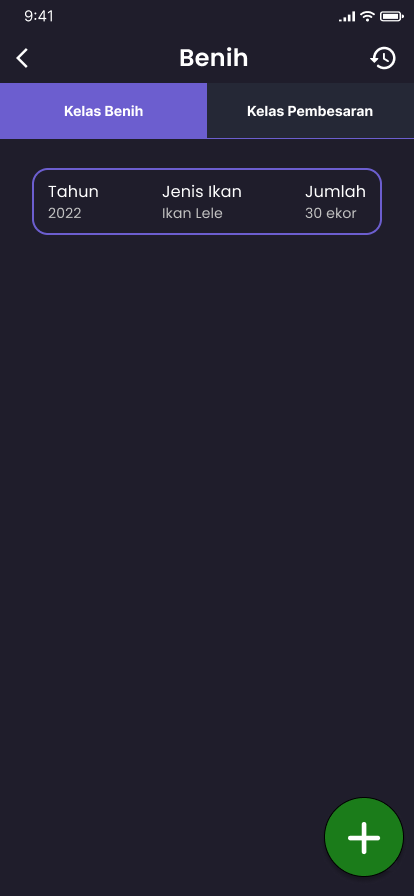
\includegraphics[width=\linewidth]{gambar/sprint1/mockup_detail_seed.png}
			  \caption{Halaman Data Inventaris Benih}
			\endminipage\hfill
			\minipage{0.32\textwidth}
			  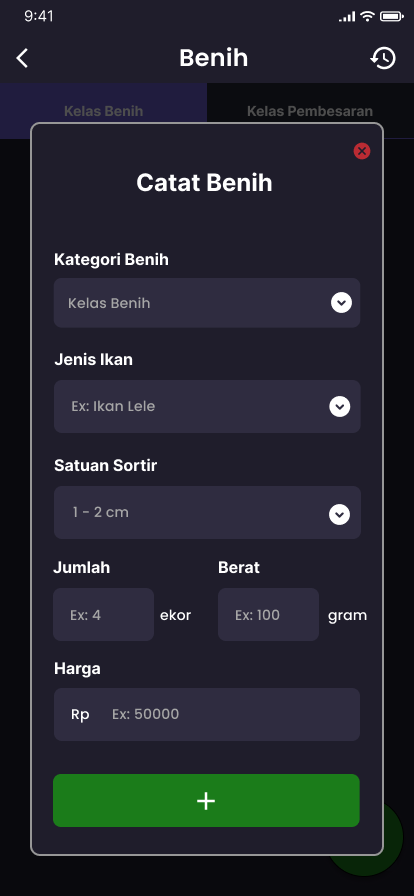
\includegraphics[width=\linewidth]{gambar/sprint1/mockup_input_seed.png}
			  \caption{Halaman Input Inventaris Benih}
			\endminipage\hfill
			\minipage{0.32\textwidth}%
			  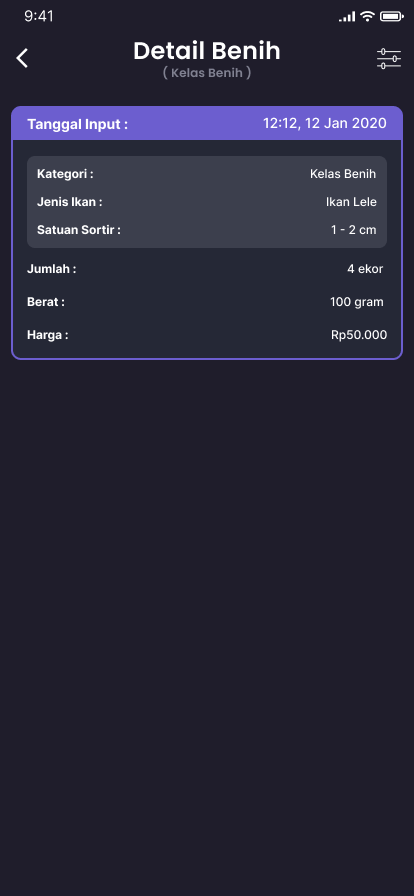
\includegraphics[width=\linewidth]{gambar/sprint1/mockup_list_seed.png}
			  \caption{Halaman Detail Inventaris Benih}
			\endminipage
		\end{figure}

		Jika pada halaman menu inventaris sebelumnya dipilih menu "Benih", maka akan masuk ke halaman data inventaris benih. Pada halaman ini terdapat list dari benih yang sudah diinput pada sistem inventaris yang terbagi menjadi dua jenis yaitu benih jenis kelas benih (kecil) dan kelas pembesaran (besar). Masing-masing data memiliki detail seperti tahun benih di input, jenis benih, dan jumlah dari benih.

		Untuk tombol (+) yang ada di pojok kanan bawah, jika ditekan akan dinavigasikan ke halaman input benih ikan. Halaman input ini memiliki form seperti pada \textbf{Gambar 3.19}. Terdapat dua jenis form yang berbeda berdasarkan ketegori yang dipilih, untuk kategori kelas benih pada bagian ukurannya menggunakan satuan sortir sementara untuk kategori kelas pembesaran menggunakan panjang dan lebar untuk ukurannya.

		\begin{figure}[H]
			\minipage{0.32\textwidth}
			  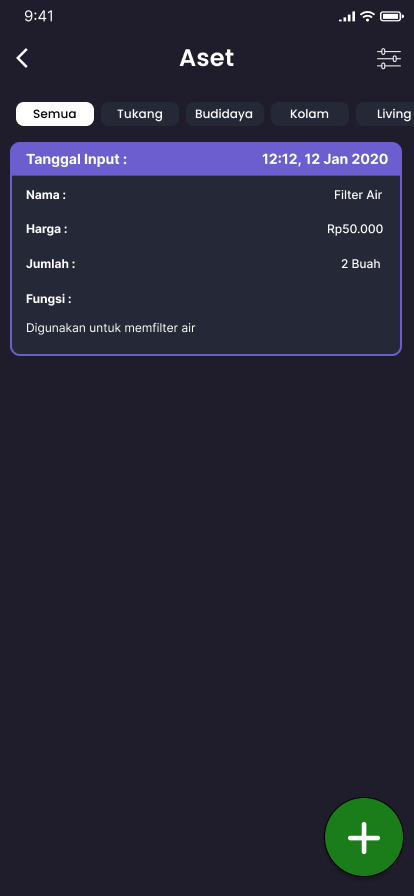
\includegraphics[width=\linewidth]{gambar/sprint1/mockup_list_aset.png}
			  \caption{Halaman Data Inventaris Aset}
			\endminipage\hfill
			\minipage{0.32\textwidth}%
			  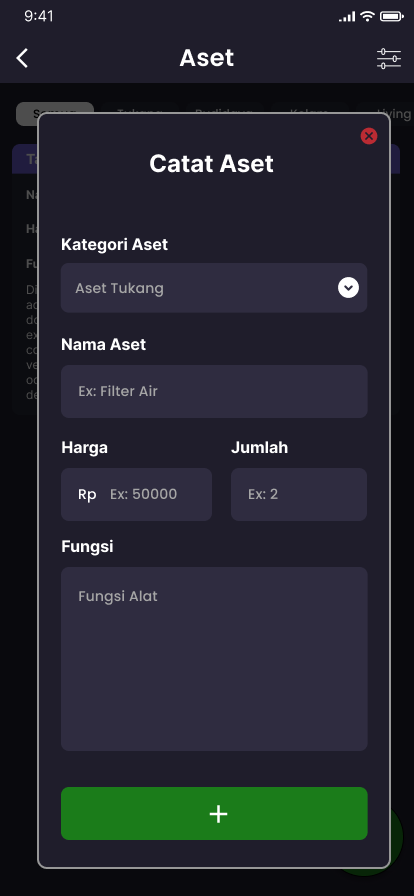
\includegraphics[width=\linewidth]{gambar/sprint1/mockup_input_aset.png}
			  \caption{Halaman Input Inventaris Aset}
			\endminipage
		\end{figure}

		Jika pada halaman menu inventaris sebelumnya dipilih menu "Aset", maka akan masuk ke halaman data inventaris aset. Pada halaman ini, ditampilkan jenis dari aset-aset yang digunakan selama masa budidaya.
		
		Aset dibagi menjadi empat jenis kategori yaitu aset tukang (aset yang diperlukan pembudidaya), aset budidaya (aset yang dibutuhkan selama budidaya berlangsung), aset kolam (aset yang digunakan dalam kolam budidaya), dan aset living (aset yang diperlukan selama berlangsungnya musim budidaya).

		Tombol (+) pada pojok kanan bawah berfungsi untuk navigasi ke halaman input sementara tombol filter pada pojok kanan atas berfungsi untuk filter data.

		\item \textbf{Sprint 2}
		
		Sprint 2 dilaksanakan pada tanggal 30 Maret 2023 - 15 April 2023. Detail dari Sprint 2 ini adalah mengerjakan tugas yang ada pada Sprint 2 Backlog di tabel berikut.
		
		\begin{table}[H]	
			\begin{center}
				\caption{Sprint 2 Backlog}
				\label{tab:table7}
				\begin{tabular}{|c|c|m{13em}|c|}
				\hline
				\textbf{No} & \textbf{Stories} & \textbf{Task} & \textbf{Status} \\
				\hline
				1 & \multirow{2}{10em}{Fitur pencatatan inventaris} & - Membuat alur UI/UX dari design aplikasi & Complete \\
				&  & - Mengupdate skema database pada inventaris & Complete \\ 
				% &  & -  & Complete \\ 
				\hline
				\end{tabular}
			\end{center}
		\end{table}

		Selama masa Sprint 2 berlangsung, tim bertemu dengan perwakilan dari Dinas Perikanan Bogor. Dari pertemuan itu, salah satunya terdapat beberapa perubahan user requirement sehingga perlu merubah skema database yang sudah dibuat pada Sprint 1. Lalu, terdapat juga pertimbangan perubahan penentuan harga jual ikan dengan ditambahkannya perhitungan aset namun hal ini belum ditentukan akan masuk perhitungan atau tidak. 

		Berikut merupakan alur user sebagai pengguna aplikasi berdasarkan mockup yang sudah dibuat pada Sprint 1.

		\begin{figure}[H]
			\centering
			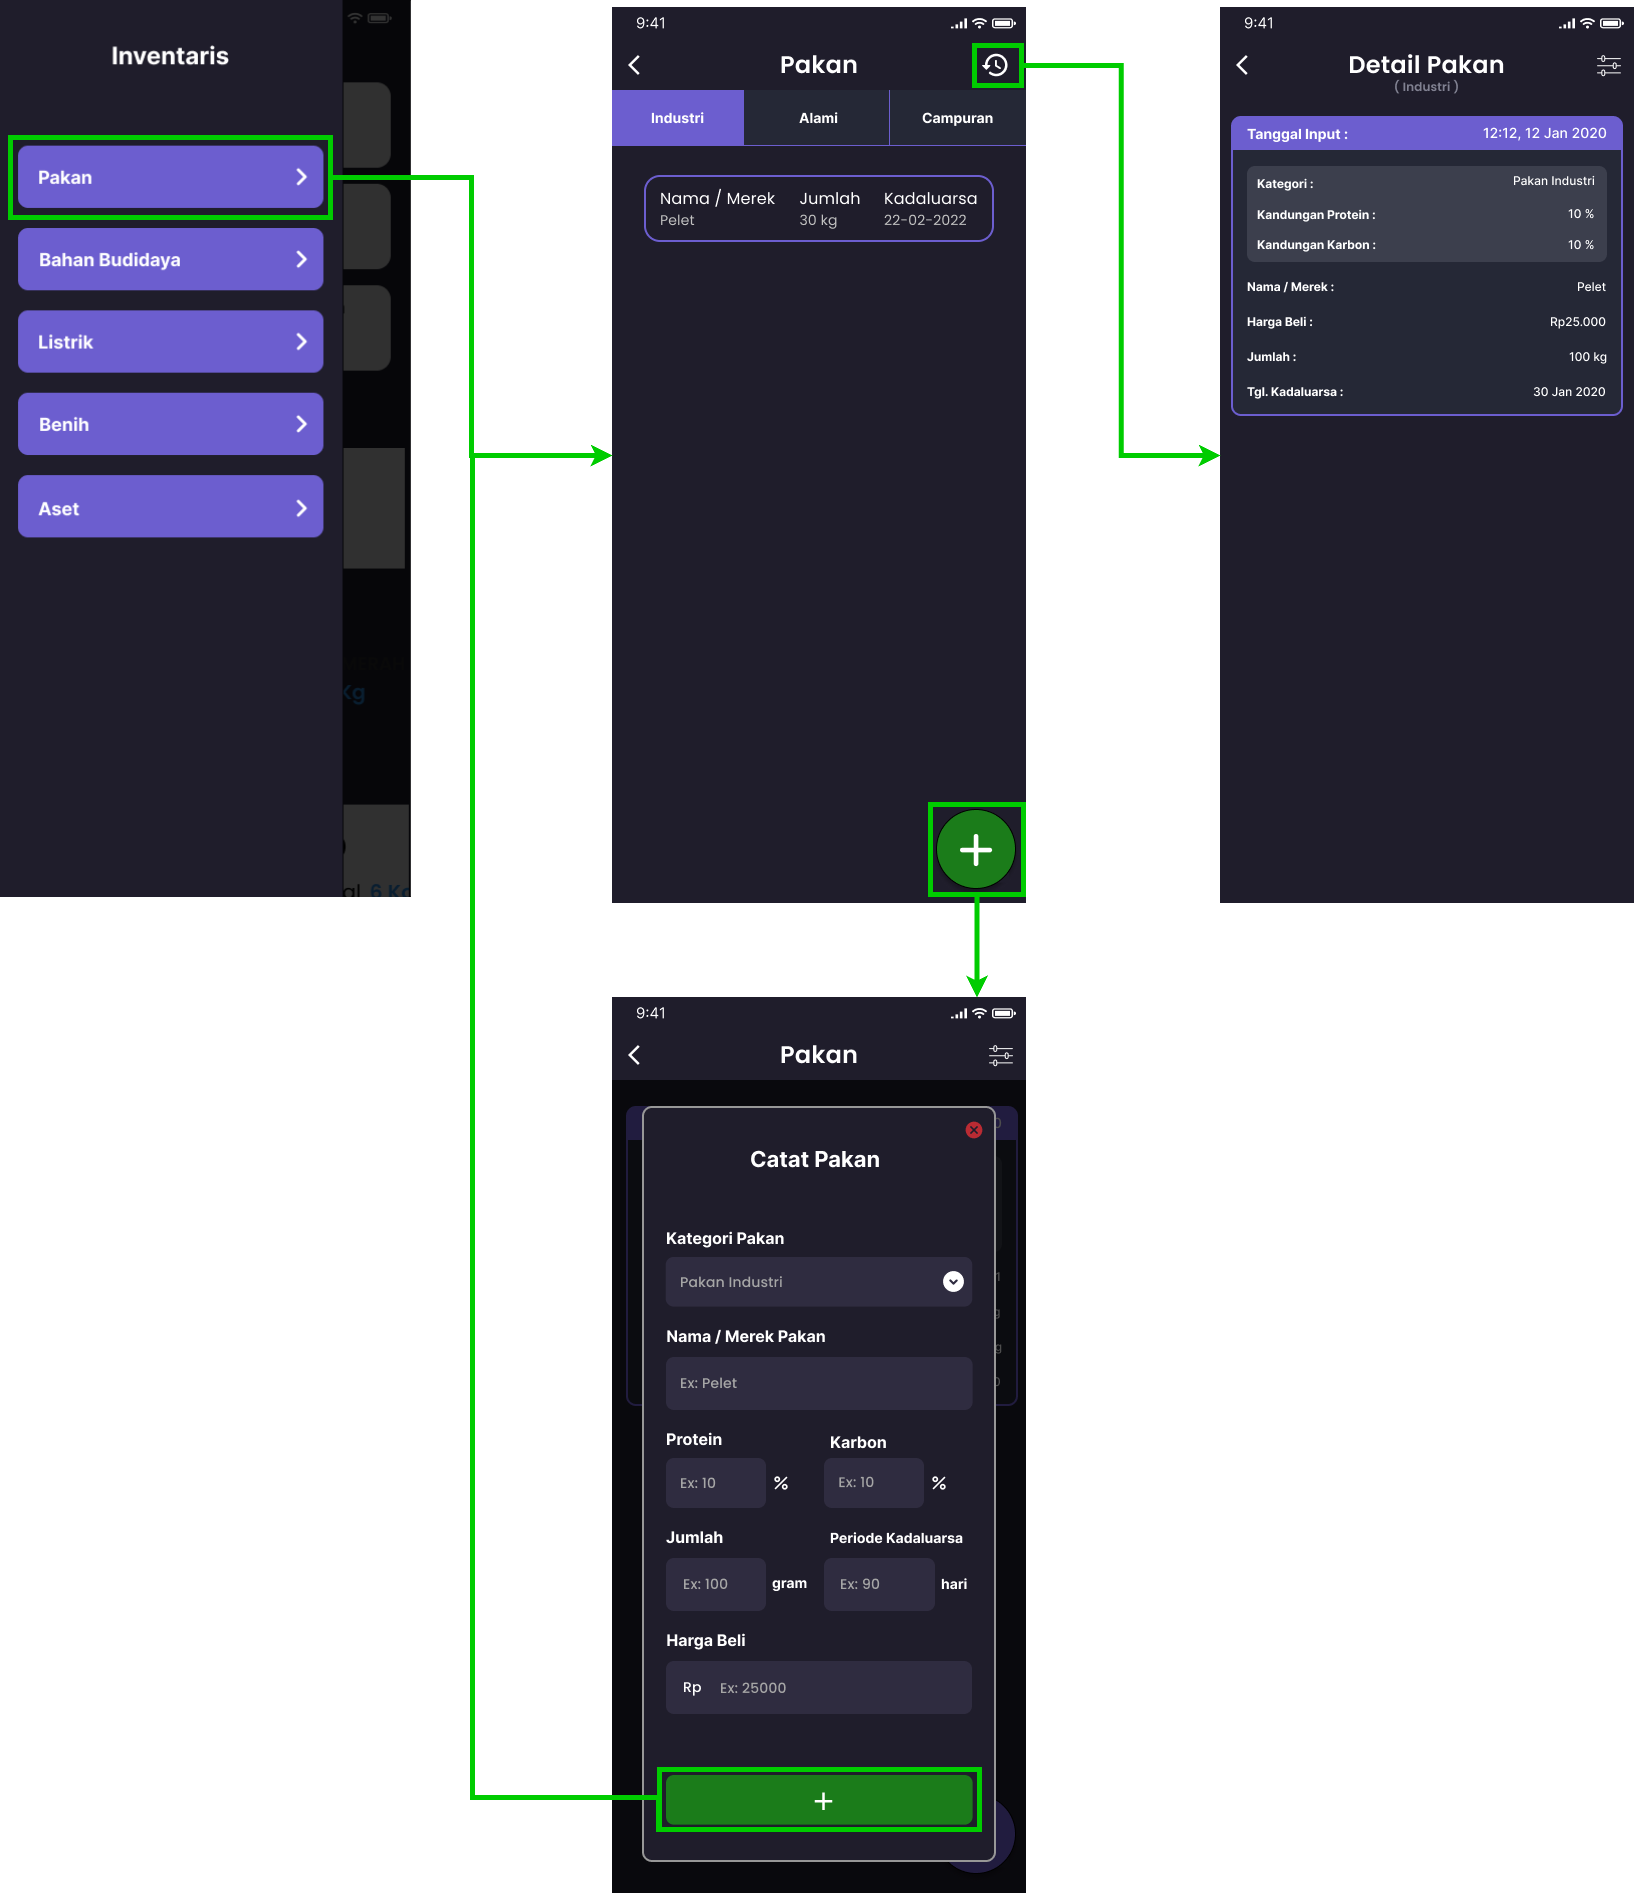
\includegraphics[width=0.9\textwidth]{gambar/sprint2/flow_feed.png}
			\caption{Alur Inventaris Pakan}
		\end{figure}

		Pada \textbf{Gambar 3.23} merupakan alur dari inventaris pakan. Pengguna akan memilih menu "Pakan" dan masuk ke halaman data inventaris pakan, kemudian tombol (+) akan menavigasikan pengguna ke halaman input pakan dan tombol riwayat akan menavigasikan pengguna ke halaman detail input pakan.

		\begin{figure}[H]
			\centering
			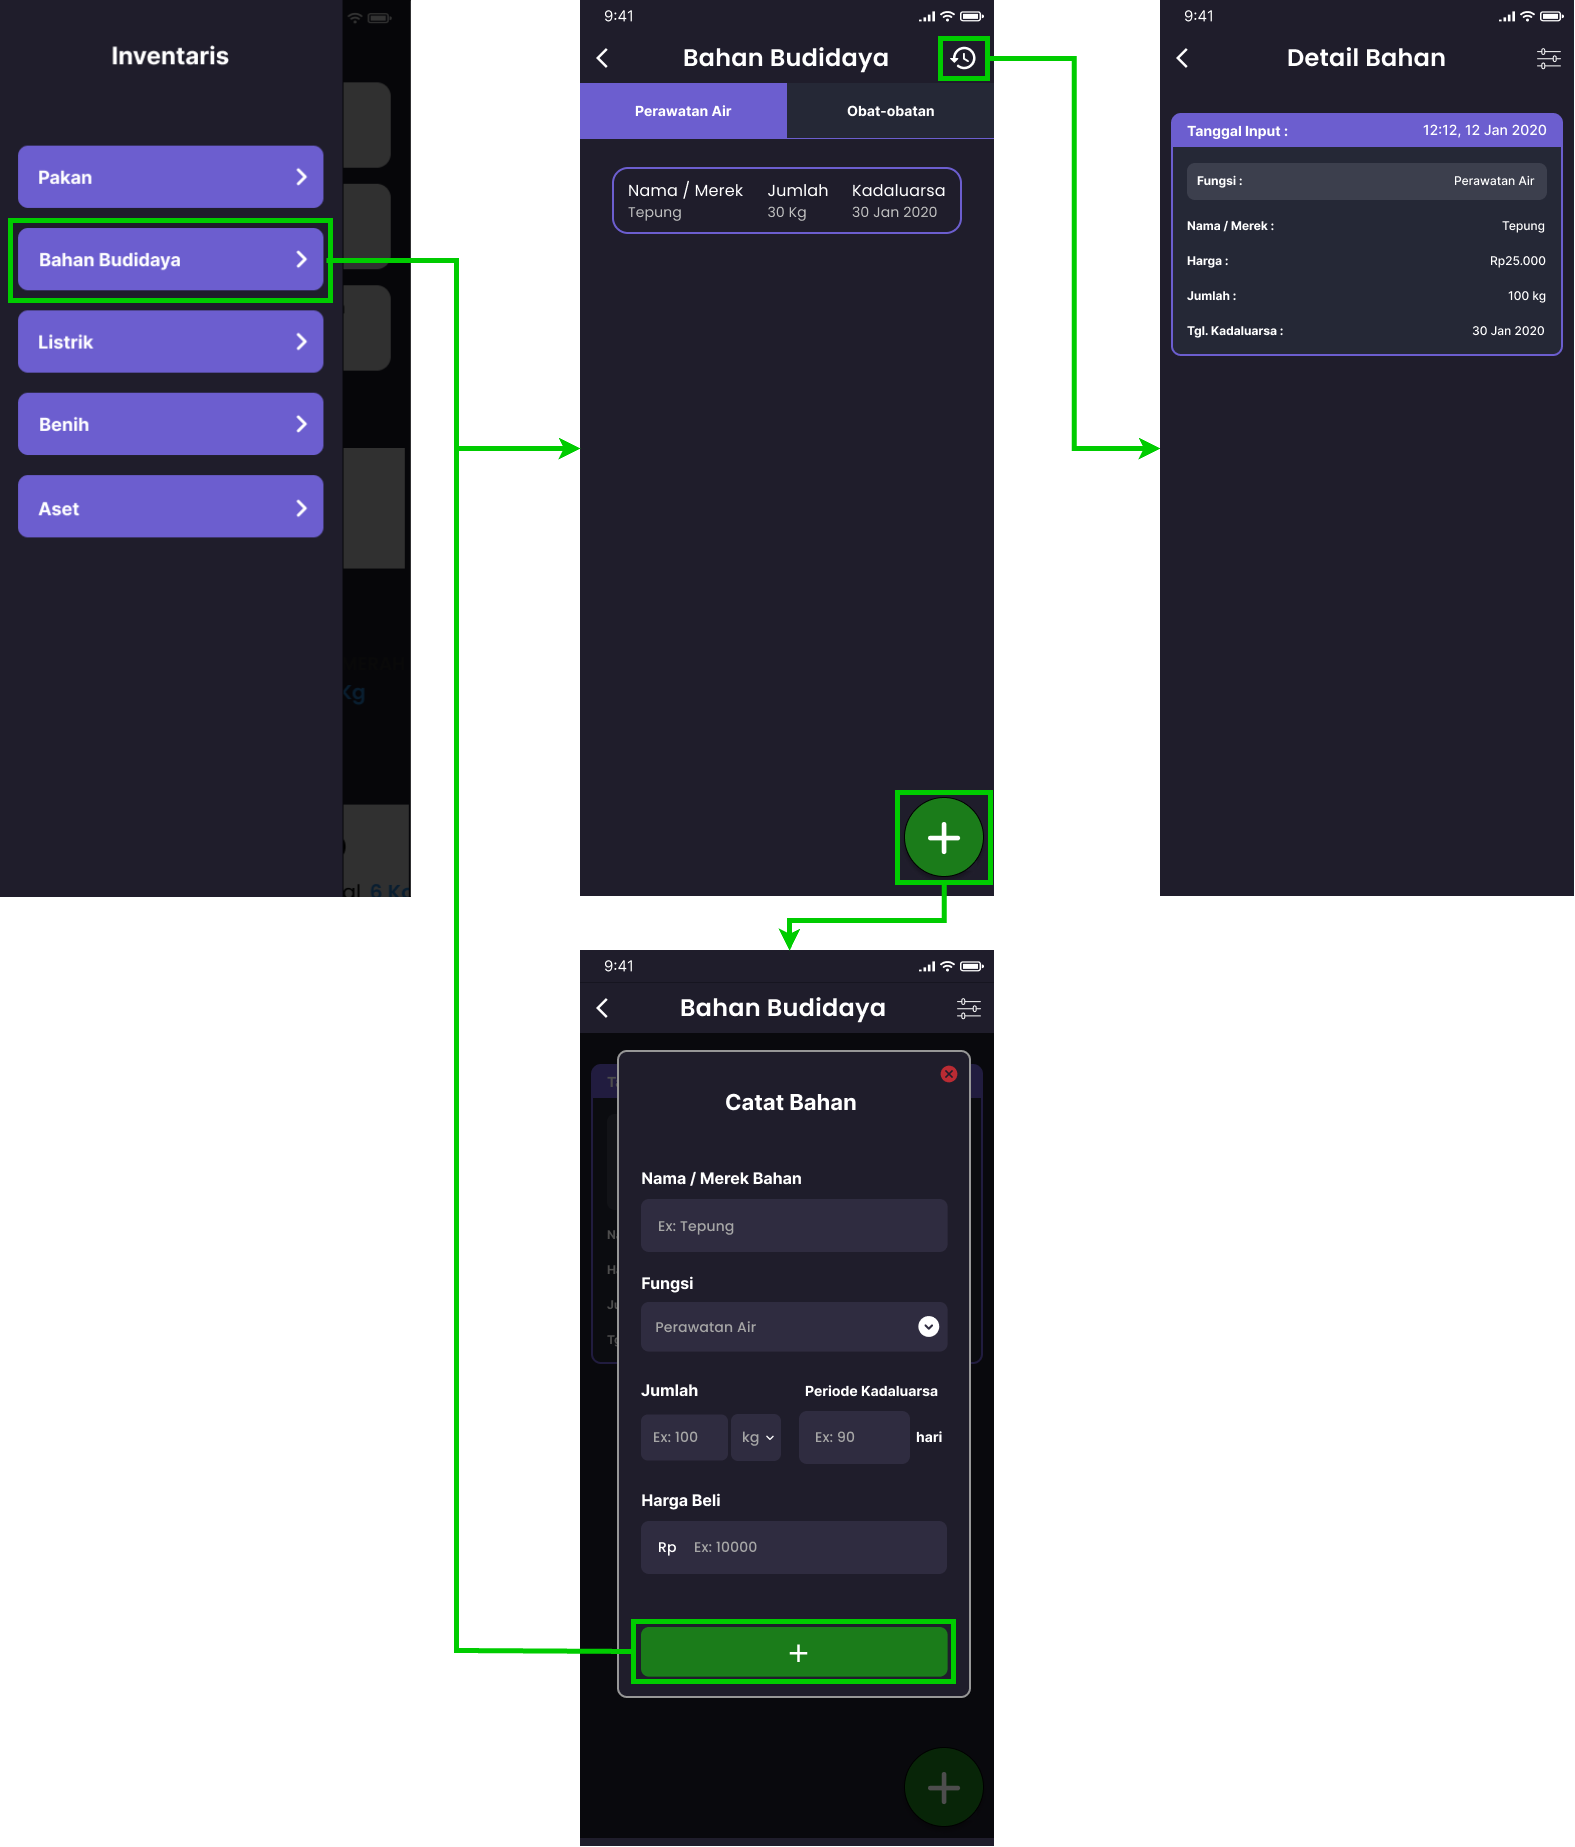
\includegraphics[width=1\textwidth]{gambar/sprint2/flow_materials.png}
			\caption{Alur Inventaris Bahan Budidaya}
		\end{figure}

		Pada \textbf{Gambar 3.24} merupakan alur dari inventaris bahan budidaya. Pengguna akan memilih menu "Bahan Budidaya" dan masuk ke halaman data inventaris budidaya, kemudian tombol (+) akan menavigasikan pengguna ke halaman input bahan budidaya dan tombol riwayat akan menavigasikan pengguna ke halaman detail input bahan budidaya.

		\begin{figure}[H]
			\centering
			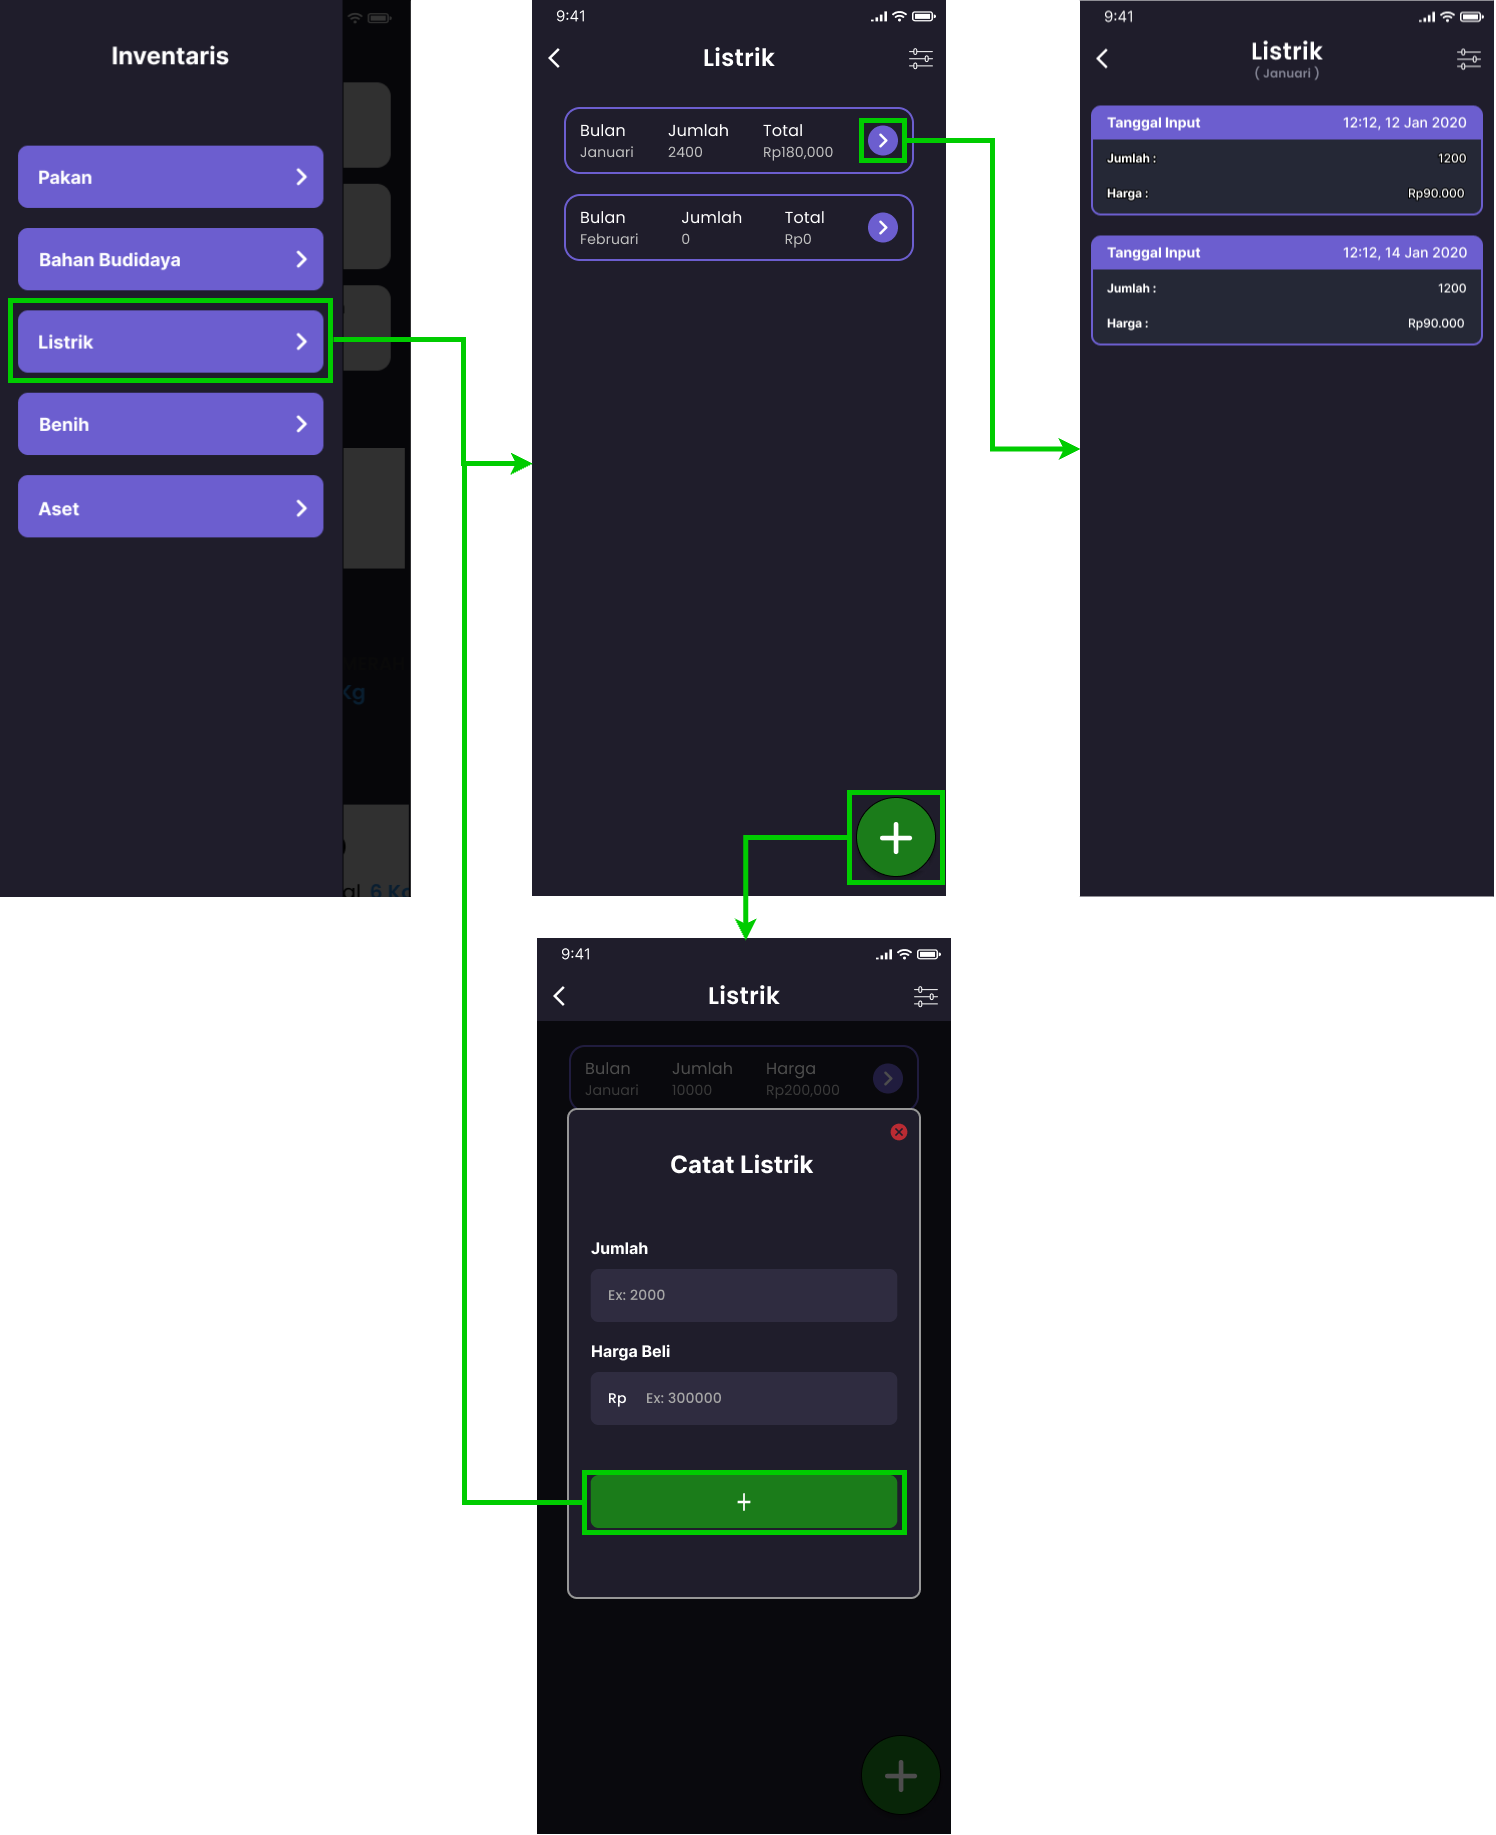
\includegraphics[width=0.9\textwidth]{gambar/sprint2/flow_electric.png}
			\caption{Alur Inventaris Listrik}
		\end{figure}

		Pada \textbf{Gambar 3.25} merupakan alur dari inventaris listrik. Pengguna akan memilih menu "Listrik" dan masuk ke halaman data inventaris listrik, kemudian tombol (+) akan menavigasikan pengguna ke halaman input listrik serta jika pengguna menekan salah satu list bulan pada data listrik, maka akan masuk ke halaman detail input tagihan listrik.

		\begin{figure}[H]
			\centering
			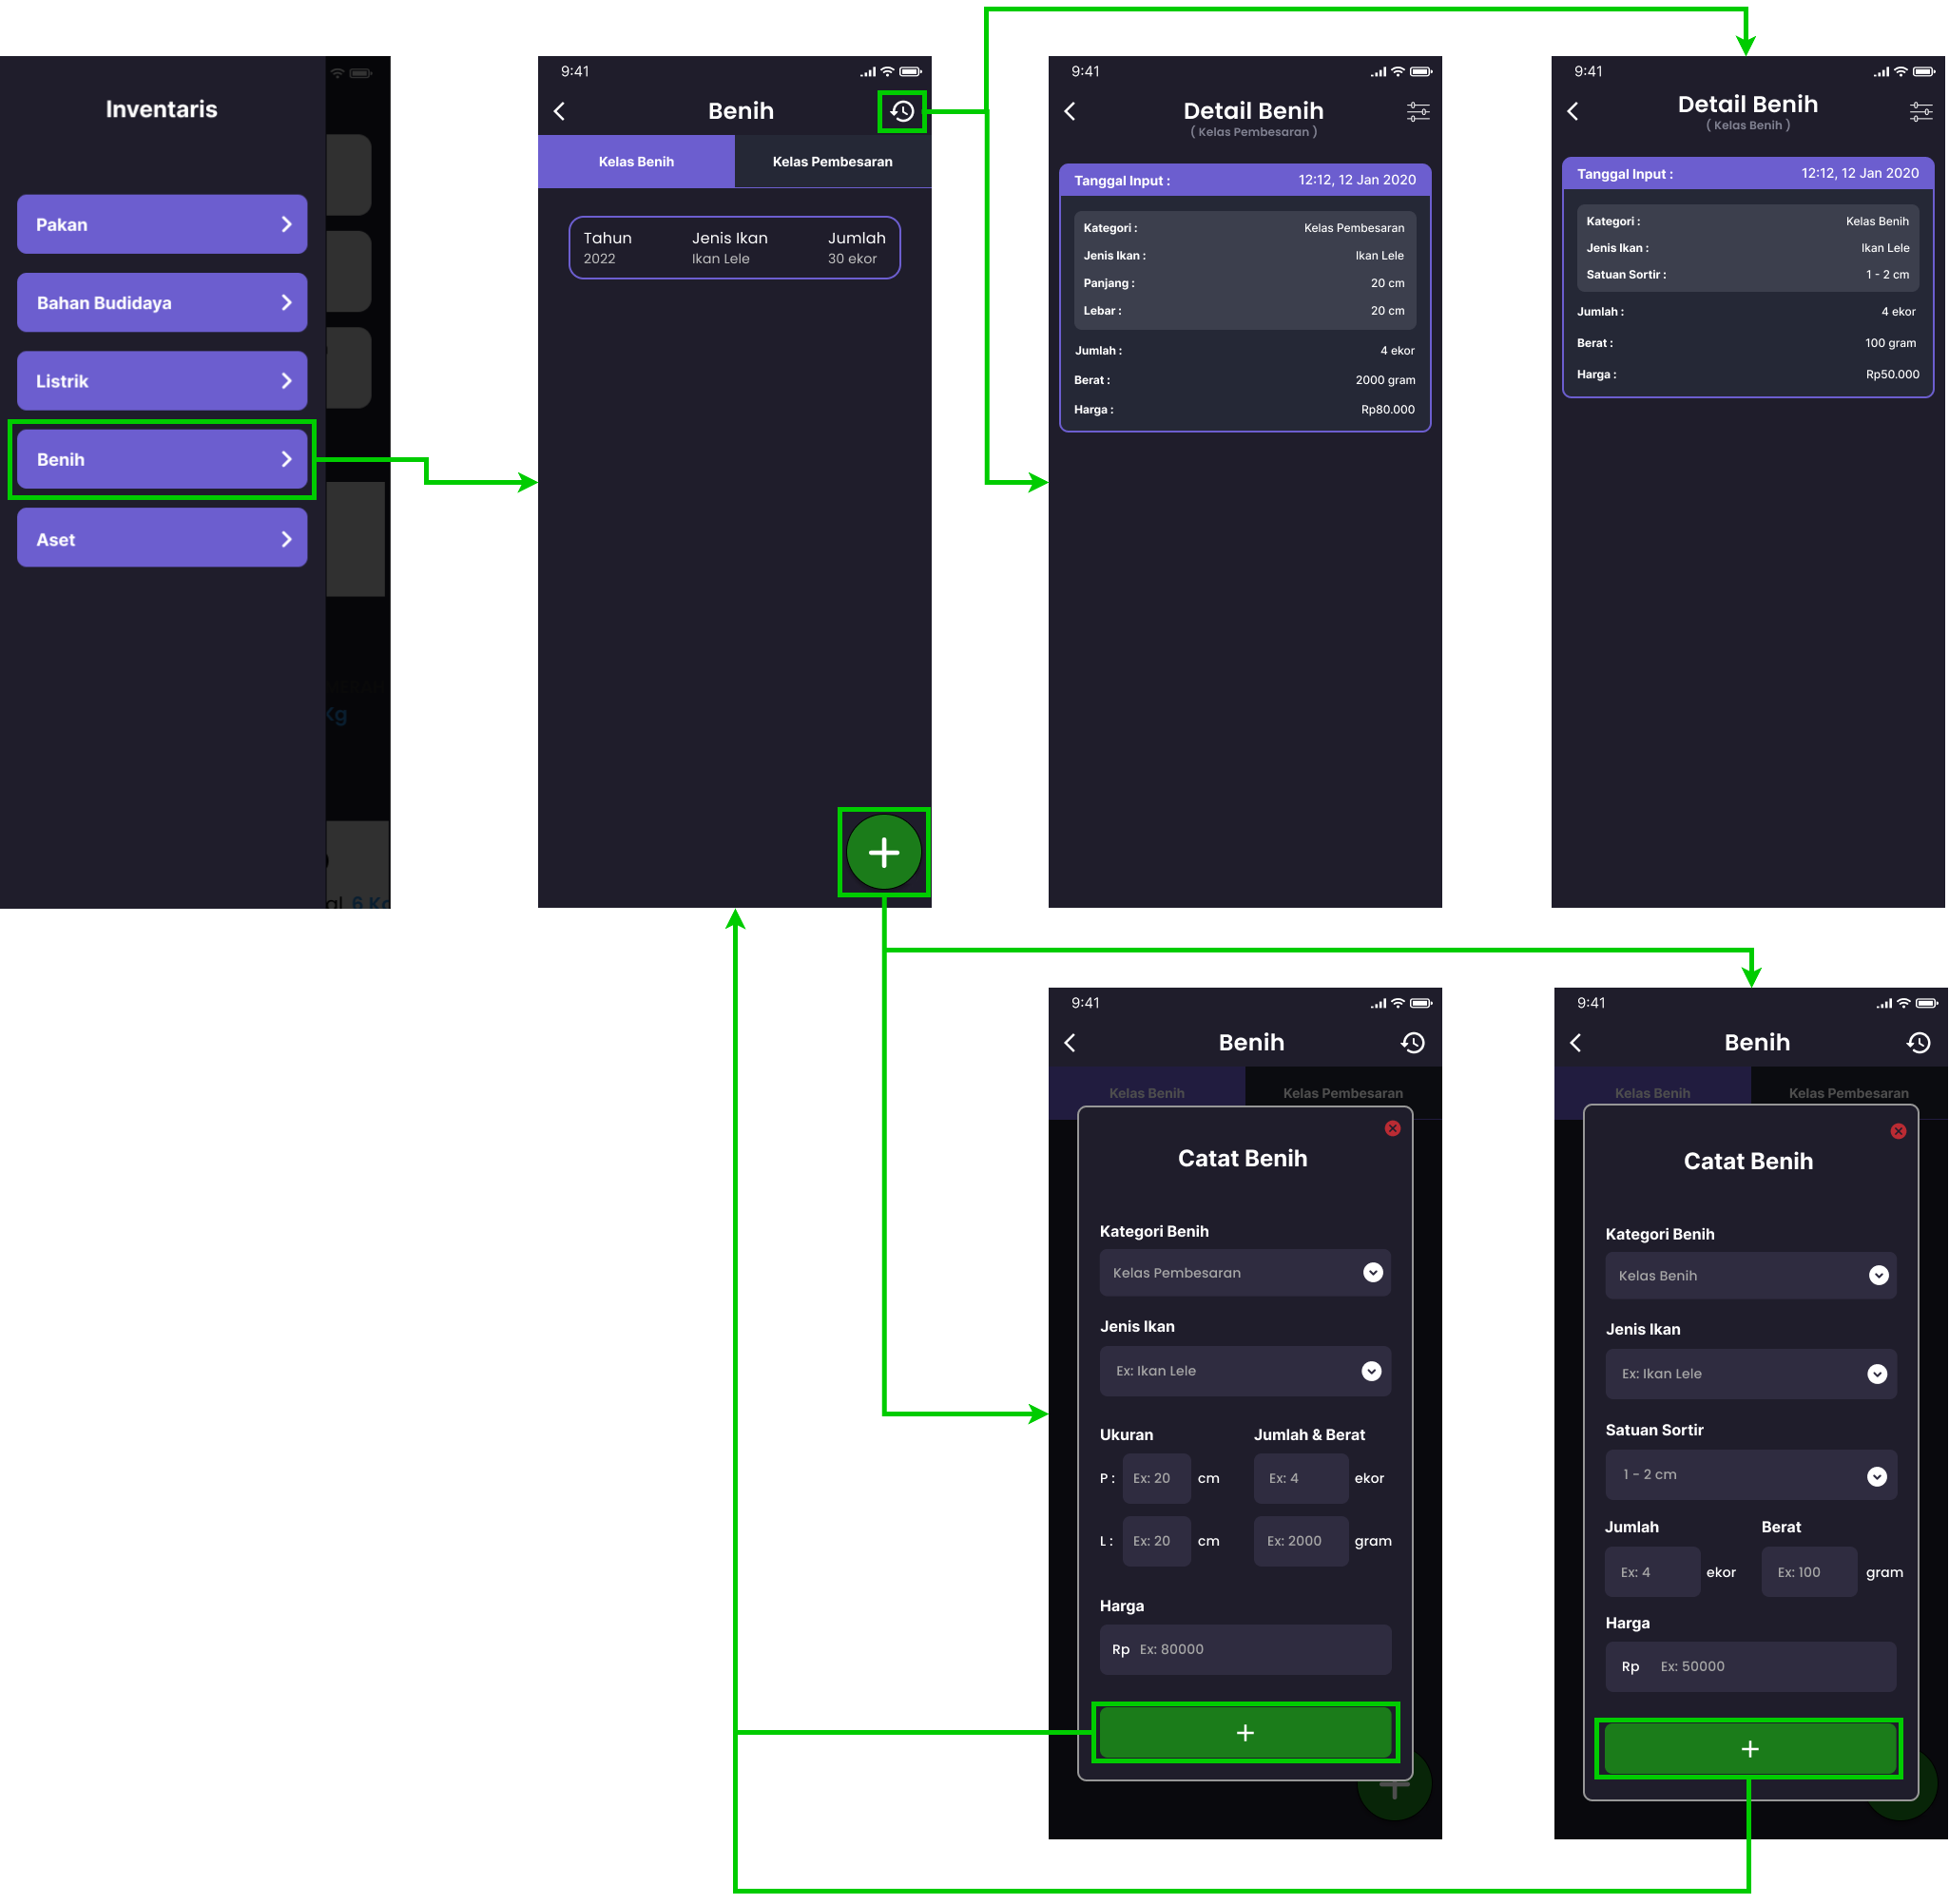
\includegraphics[width=1\textwidth]{gambar/sprint2/flow_seed.png}
			\caption{Alur Inventaris Benih}
		\end{figure}

		Pada \textbf{Gambar 3.26} merupakan alur dari inventaris benih. Pengguna akan memilih menu "Benih" dan masuk ke halaman data inventaris benih, kemudian tombol (+) akan menavigasikan pengguna ke halaman input benih dan tombol riwayat akan menavigasikan pengguna ke halaman detail input benih.

		\begin{figure}[H]
			\centering
			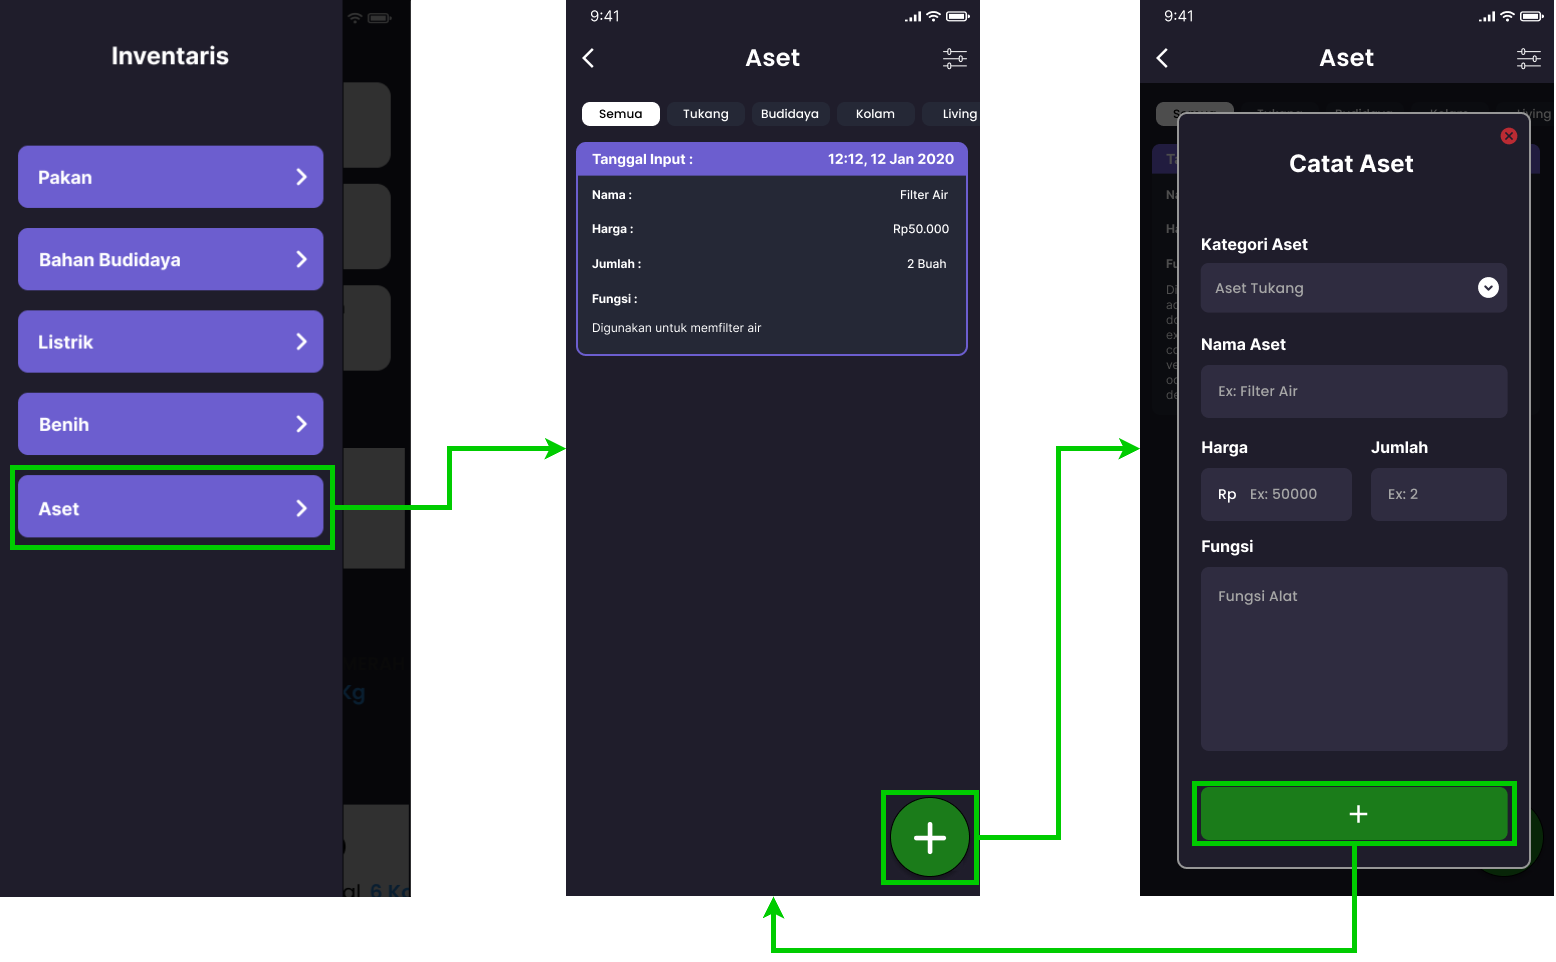
\includegraphics[width=1\textwidth]{gambar/sprint2/flow_asset.png}
			\caption{Alur Inventaris Aset}
		\end{figure}

		Pada \textbf{Gambar 3.27} merupakan alur dari inventaris aset. Pengguna akan memilih menu "Aset" dan masuk ke halaman data inventaris aset, kemudian tombol (+) akan menavigasikan pengguna ke halaman input aset.

		Seteleh semua alur telah selesai dibuat, selanjutnya merupakan perubahan skema database inventaris yang dapat dilihat pada \textbf{Gambar 3.28} berikut.

		\begin{figure}[H]
			\centering
			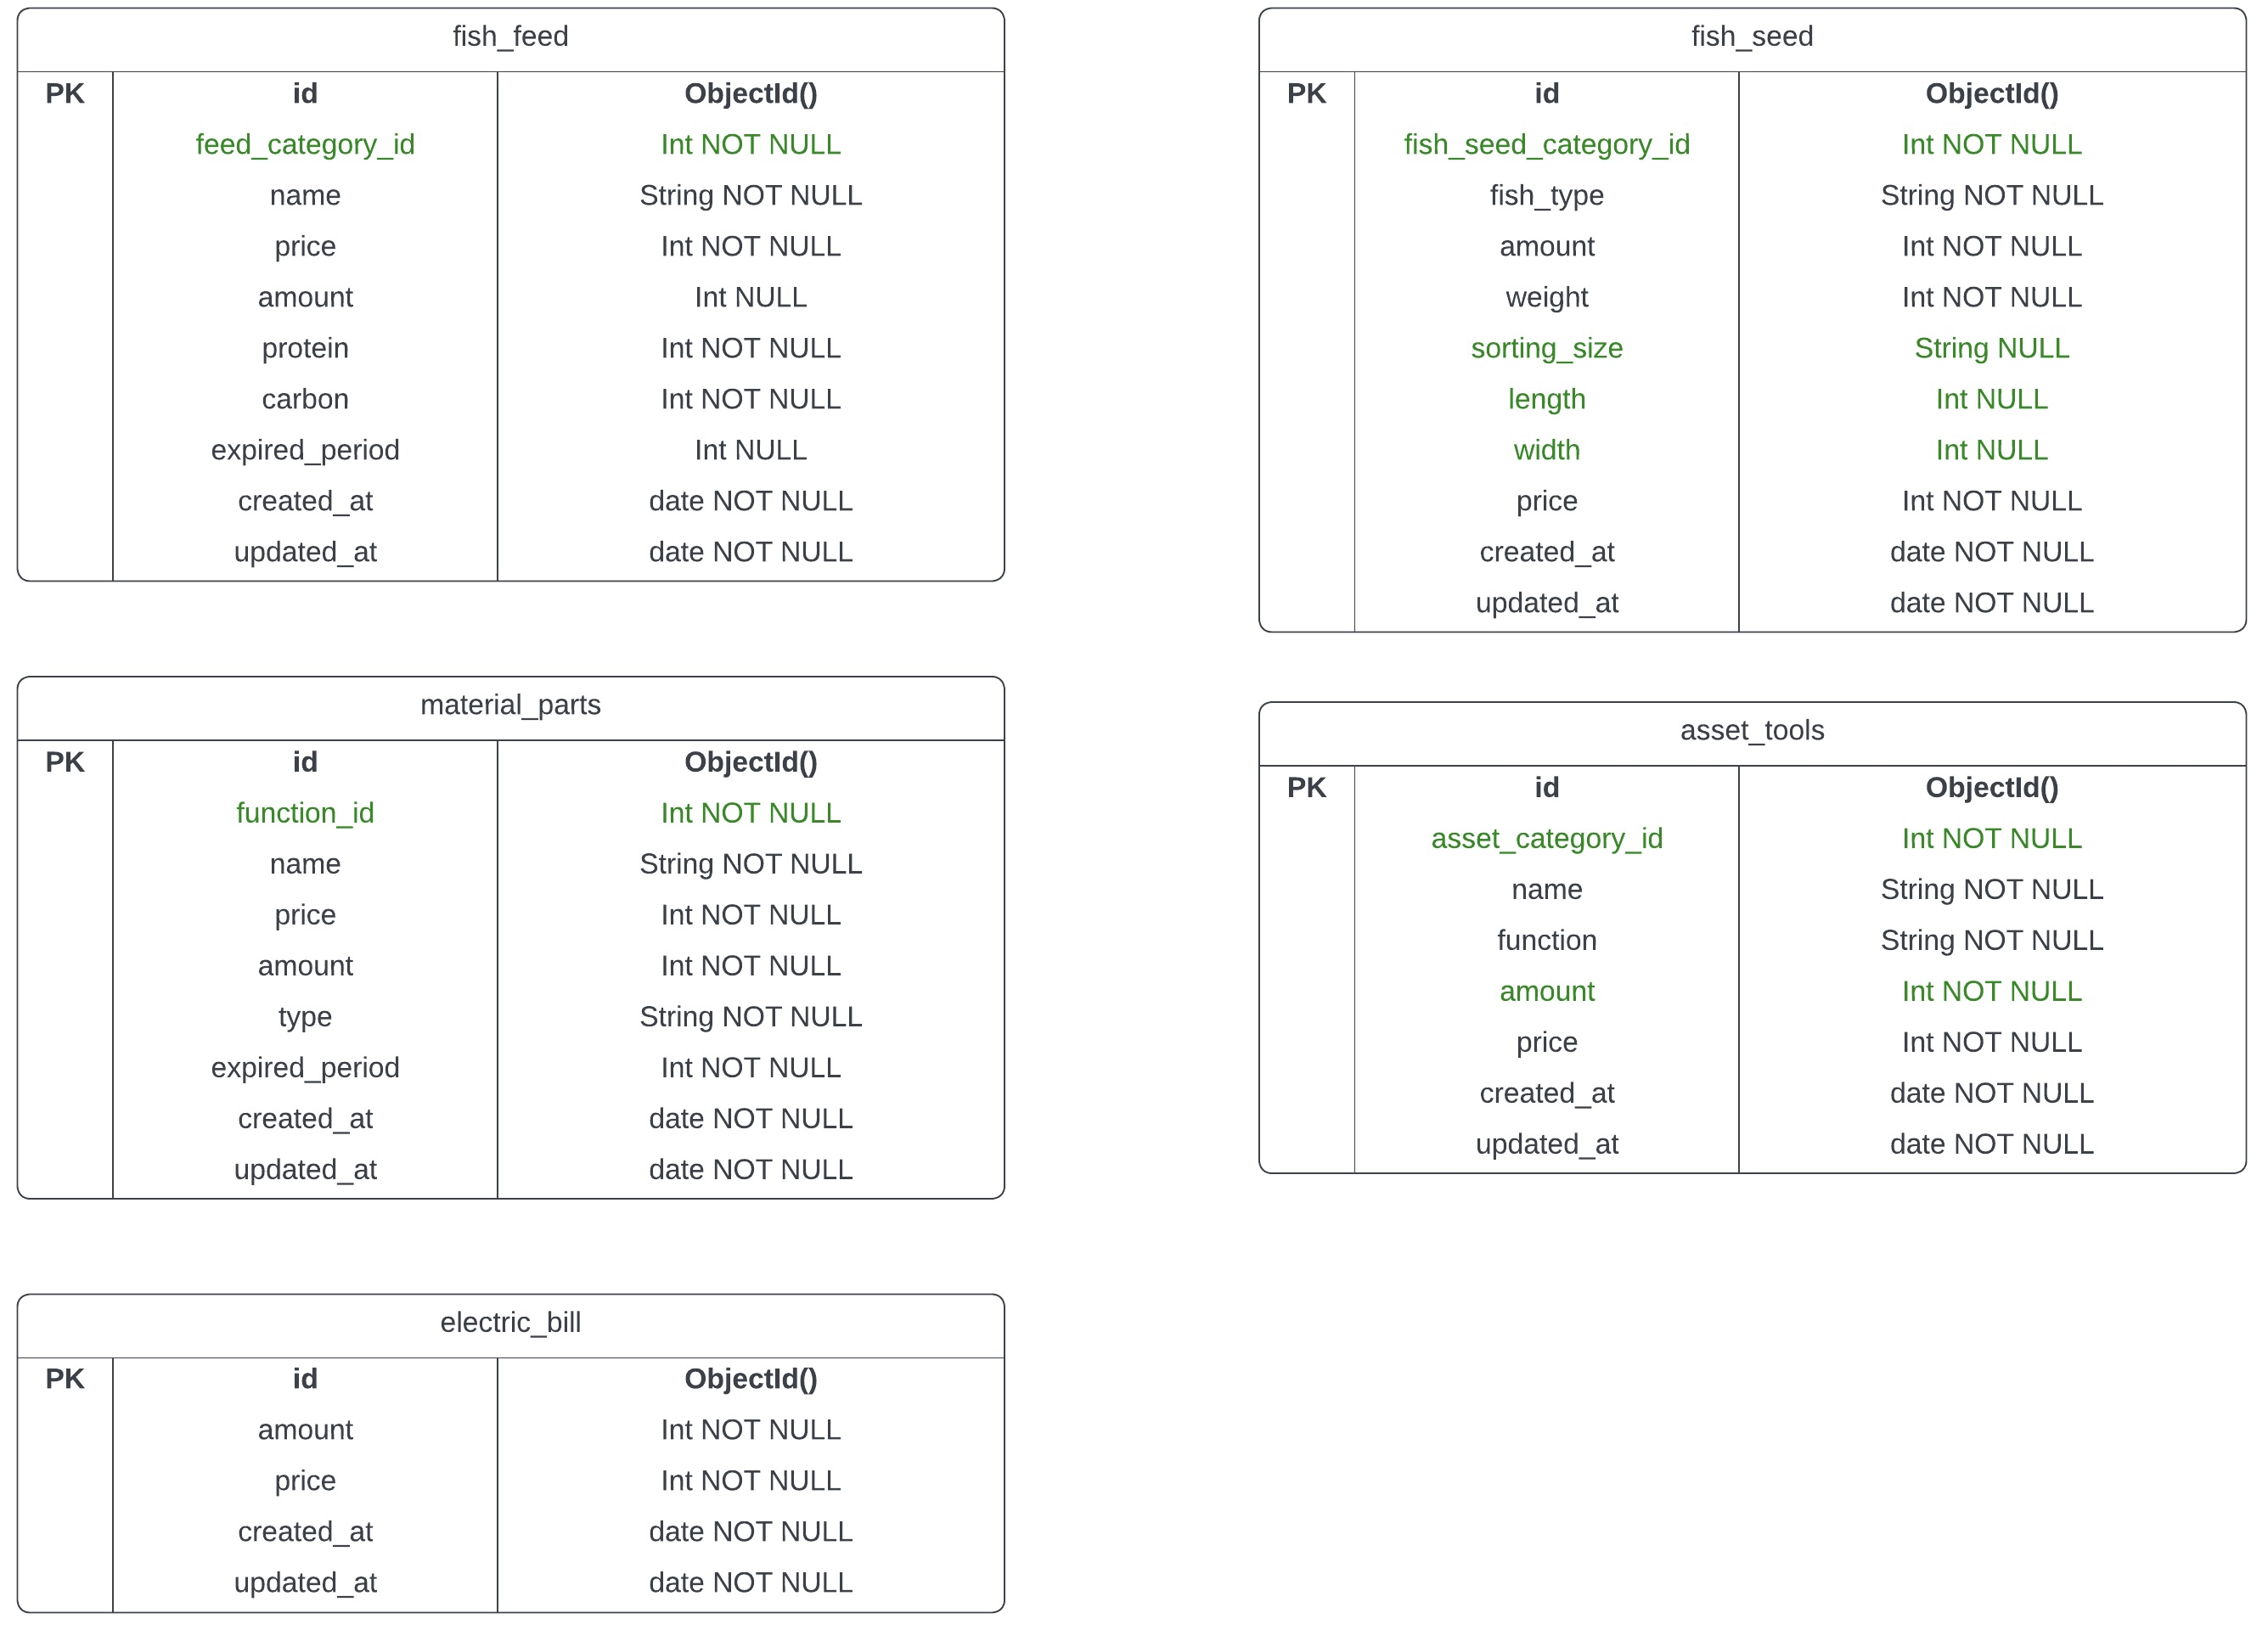
\includegraphics[width=1\textwidth]{gambar/sprint2/inventory_schema.jpeg}
			\caption{Update Skema Database Inventaris}
		\end{figure}

		Berdasarkan skema database inventaris tersebut, jika dibandingkan dengan skema database inventaris sebelumnya pada \textbf{Gambar 3.5} terdapat pembaruan pada bagian inventaris pakan, bahan budidaya, benih, dan aset.

		Pada skema database di inventaris pakan (fish\_feed), ditambahkan \textit{key} \textbf{feed\_category\_id} karena pada inventaris pakan diharuskan memilih kategori pakan yang akan dimasukkan. Untuk itu feed\_category\_id berperan untuk menampung jenis kategori pakan yang akan diinput. Sebelumnya jenis inventaris pakan tidak memiliki kategori, sehingga perlu ditambahkan \textit{key} baru untuk jenis data kategori tersebut.

		Kemudian, di skema database inventaris bahan budidaya (material\_parts) ditambahkan \textit{key} \textbf{function\_id} karena bahan budidaya dibagi menjadi dua fungsi yaitu perawatan air dan obat-obatan. Sebelumnya inventaris bahan budidaya tidak memiliki kategori, sehingga harus ditambahkan \textit{key} baru pada database untuk menampung jenis data tersebut.

		Lalu pada skema database inventaris benih ditambahkan \textit{key} \textbf{fish\_seed\_category\_id}, \textbf{sorting\_size}, \textbf{length}, serta \textbf{width}. \textit{key} tersebut ditambahkan karena pada benih dibagi menjadi dua jenis yaitu kelas benih dan kelas pembesaran. Masing-masing kategori memiliki jenis data pengukuran yang berbeda, pada kelas benih digunakan pengukuran satuan sortir dengan \textit{key} sorting\_size sementara kelas pembesaran digunakan pengukuran panjang dan lebar dengan \textit{key} \textit{length} dan \textit{width}. Sebelumnya untuk benih tidak terdapat kategori dan jenis ukuran benih sehingga \textit{key} baru diperlukan untuk menampung data tersebut.

		Terakhir terdapat perubahan pada skema database inventaris aset yaitu ditambahkan \textit{key} \textbf{asset\_category\_id} dan \textbf{amount}. Sebelumnya inventaris aset hanya menampung segala jenis aset yang digunakan pada musim budidaya tanpa adanya jenis kategori dan jumlah yang spesifik, namun di skema database sekarang dapat ditentukan jenis kategori pada aset dan berapa jumlah aset yang digunakan sehingga pemantauan aset yang digunakan menjadi lebih detail.

	\end{enumerate}
	
	\item Sprint Review
	
	Setelah Sprint berjalan, setiap minggunya diadakan meet bersama tim untuk melaksanakan Sprint Review yang bertujuan untuk melaporkan perkembangan Sprint baik itu proses ataupun hambatan selama pengerjaan Sprint.
	
	\item Deploy Sistem
	
	Ketika semua task sprint yang ada di sprint backlog selesai, maka aplikasi akan di deploy untuk dijalankan pengujian pada aplikasi. Pengujian aplikasi ini dilakukan dengan menggunakan Unit Testing dan User Analytics.
	
\end{enumerate}

\section{Pengujian}

Di tahap pengujian ini, peneliti akan melakukan uji aplikasi menggunakan dua jenis pengujian yaitu unit testing dan User Acceptance Test (UAT). Pengujian unit testing dilakukan oleh tim internal developer aplikasi untuk memastikan kepastian fungsi fitur dan cara kerja fitur agar aplikasi sesuai dengan kebutuhan. Sementara UAT dilakukan oleh user untuk mengetahui apakah aplikasi sudah memenuhi kebutuhan dan layak digunakan.

\begin{enumerate}
	\item Unit Testing
	
	Pengujian dengan unit testing ini dibuat berdasarkan product backlog dan daftar sprint-sprint backlog yang sudah selesai. Pengujian internal ini mengubah status Complete pada task di Sprint Backlog menjadi Tested. Berikut skenario pengujian yang akan dilakukan dapat dilihat pada \textbf{Tabel 3.4} berikut.

	\begin{table}[H]	
		\begin{center}
			\caption{Skenario Unit Testing}
			\label{tab:table8}
			\begin{tabular}{|m{13em}|m{17em}|}
			\hline
			\textbf{Jenis Fitur} & \textbf{Skenario Pengujian} \\
			\hline
			Pencatatan Inventaris & Saat aplikasi dibuka dan sudah terautentikasi, halaman dashboard akan tampil \\
			\hline
			 & Di halaman dashboard, terdapat tombol list yang ada pada pojok kiri atas aplikasi \\
			\hline
			 & Jika tombol list ditekan, maka akan tampil beberapa list menu inventaris \\
			\hline
			& Ketika salah satu tombol pada list inventaris ditekan, maka akan masuk ke halaman detail data inventaris dari menu yang dipilih \\
			\hline
			& Pada halaman detail data inventaris, ketika tombol riwayat di pojok kanan atas ditekan akan muncul rincian input pada sistem inventaris \\
			\hline
			& Pada halaman detail data inventaris, Ketika tombol (+) yang ada di pojok kanan bawah ditekan akan masuk ke halaman input data inventaris \\
			\hline
			Pencatatan Inventaris (Listrik dan Aset) & Khusus untuk inventaris listrik dan aset, dipojok kanan atas halaman detail data inventaris terdapat tombol filter yang jika ditekan akan memfilter data inventaris berdasarkan jenis filter yang dipilih  \\
			\hline
			\end{tabular}
		\end{center}
	\end{table}

	\item User Analytics
	
	Pengujian ini dilakukan kepada pembudidaya ikan dengan 3 tahap yaitu tutorial, logging / survei penggunaan aplikasi, dan interview. Tahapan tersebut dilakukan secara bertahap dan masing-masing tahap dijelaskan seperti berikut.

	\begin{enumerate}
		\item Tahap Tutorial
		
		Pada tahap ini, dilakukan sesi pertemuan dengan para pembudidaya untuk menjelaskan fitur-fitur yang ada pada aplikasi secara keseluruhan.

		\item Tahap Logging
		
		Pada tahap ini, setiap aktivitas aplikasi yang dilakukan oleh pembudidaya akan dicatat oleh sistem. Hal ini mencakup seperti detail halaman yang diakses dan detail penggunaan fitur yang ada.
	
		\item Tahap Interview
		
		Pada tahap ini, terdapat sesi interview dengan pembudidaya mengenai penggunaan aplikasi. Dapat ditanyakan detail dari penggunaan aplikasi berdasarkan data logging yang sudah dikumpulkan sebelumnya.
	\end{enumerate}

	% \item User Acceptance Test (UAT)
	
	% Pengujian dengan User Acceptance Test dibuat berdasarkan fitur yang bisa diakses oleh user pada product backlog yang ada pada \textbf{Tabel 3.1}. Untuk skenario pengujiannya dapat dilihat pada \textbf{Tabel 3.5} berikut.

	% \begin{table}[H]	
	% 	\begin{center}
	% 		\caption{Tabel Skenario UAT}
	% 		\label{tab:table9}
	% 		\begin{tabular}{|m{10em}|m{14em}|m{5em}|}
	% 		\hline
	% 		\textbf{Jenis Fitur} & \textbf{Skenario Pengujian} & \textbf{Jenis Pengujian} \\
	% 		\hline
	% 		Pencatatan Inventaris & Menekan tombol list pada halaman dashboad dan memilih menu inventaris yang ada pada list, kemudian menekan tombol (+) untuk menambahkan data serta tombol riwayat untuk melihat rincian input inventaris & UAT \\
	% 		\hline
	% 		%  & Di halaman dashboard, terdapat tombol list yang ada pada pojok kiri atas aplikasi \\
	% 		% \hline
	% 		%  & Jika tombol list ditekan, maka akan tampil beberapa list menu inventaris \\
	% 		% \hline
	% 		% & Ketika salah satu tombol pada list inventaris ditekan, maka akan masuk ke halaman detail data inventaris dari menu yang dipilih \\
	% 		% \hline
	% 		% & Pada halaman detail data inventaris, ketika tombol riwayat di pojok kanan atas ditekan akan muncul rincian input pada sistem inventaris \\
	% 		% \hline
	% 		% & Pada halaman detail data inventaris, Ketika tombol (+) yang ada di pojok kanan bawah ditekan akan masuk ke halaman input data inventaris \\
	% 		% \hline
	% 		% Pencatatan Inventaris (Listrik dan Aset) & Khusus untuk inventaris listrik dan aset, dipojok kanan atas halaman detail data inventaris terdapat tombol filter yang jika ditekan akan memfilter data inventaris berdasarkan jenis filter yang dipilih  \\
	% 		% \hline
	% 		\end{tabular}
	% 	\end{center}
	% \end{table}	
\end{enumerate}

% \subsection*{Daily Scrum}

% Daily Scrum merupakan kegiatan rutin tiap minggu yang dilaksanakan dengan Scrum Master. Kegiatan ini dilakukan untuk reporting progres tugas yang dijalankan selama masa Sprint berlangsung kepada Scrum Master. Scrum Master bertugas untuk memberikan feedback saat Daily Scrum berlangsung.

% \subsection*{Sprint Review dan Sprint Restropective}

% Sprint Review dan Sprint Restropective adalah kegiatan mengulas kembali tugas yang sudah dikerjakan pada saat durasi Sprint berlangsung. Kegiatan ini juga merupakan kegiatan menentukan tugas yang berhasil dan tidak berhasil selama Sprint berlangsung